% PAKETE UND DOKUMENTKONFIGURATION
\documentclass[11pt, a4paper]{article}

% Encoding für Umlaute
\usepackage[utf8]{inputenc}
\usepackage[T1]{fontenc}

% Silbentrennung
\usepackage[ngerman]{babel}

% erweiterte Matheumgebungen und Formelnummer mit Sectionnummer
\usepackage{amsmath}
\numberwithin{equation}{section}

% Braket Notation
\usepackage{braket}
\usepackage{isotope}

% zusätzliche mathematische Schriftarten
\usepackage{amsfonts}

% verschiedene mathematische Symbole
\usepackage{amssymb}

% Einheiten setzen z.B. \SI{10}{\kilo\gram\meter\per\second\squared}
% Fehler: \SI{10 +- 0,2e-4}{\metre}
\usepackage{siunitx}
\sisetup{
  output-decimal-marker={,},
  separate-uncertainty
}

% Einheitendefinitionen
\DeclareSIUnit{\skt}{Skt.}
\DeclareSIUnit{\gauss}{G}

% Operatordefinitionen
\DeclareMathOperator{\erf}{erf}

% Randbreiten
\usepackage[left=3.5cm,right=3.5cm,top=3cm,bottom=3cm,twoside]{geometry}

% Bilder einfügen
\usepackage{graphicx}

% Verweise innerhalb des Dokuments
\usepackage{hyperref}
\hypersetup{
	colorlinks = true,
	allcolors = {black}
}

% bessere Tabellenlayouts
\usepackage{booktabs}
\usepackage{multirow}
\usepackage{multicol}

% Seitenlayout (Kopfzeile)
\usepackage{fancyhdr}

% Float Barriers
\usepackage{placeins}

% Pakete für gedrehte Subfigures
\usepackage{caption}
\usepackage{subcaption}
\usepackage{rotating}

% Paket für textumflossene Abbildungen und Tabellen
\usepackage{wrapfig}


% Caption-Setup
\captionsetup{font={small}}
\renewcommand{\thefigure}{\thesection.\arabic{figure}}
\renewcommand{\thesubfigure}{\alph{subfigure}}
\renewcommand{\thetable}{\thesection.\arabic{table}}
\renewcommand{\thesubtable}{\alph{subtable}}

% Manuelle Silbentrennung
\hyphenation{Re-so-na-tor Mo-den-ab-stand Re-so-na-tor-län-ge}

% Tiefe des Inhaltsverzeichnisses (Level: 1 sections, 2 subsections,
% 3 subsubsections)
\setcounter{tocdepth}{3}

% FANCYHDR SETUP
\pagestyle{fancy}
\fancyhead[EL,OR]{\thepage}
\fancyhead[ER]{\leftmark}
\fancyhead[OL]{\rightmark}

\renewcommand{\sectionmark}[1]{
\markboth{\thesection{} #1}{\thesection{} #1}
}
\renewcommand{\subsectionmark}[1]{
\markright{\thesubsection{} #1}
}

% DOKUMENTINFORMATIONEN
\title{P523 \\ Beta Spektrometer}

\author{Christopher Deutsch\footnote{christopher.deutsch@uni-bonn.de} \and Christian Bespin\footnote{christian.bespin@uni-bonn.de}}

\date{\today}

\begin{document}

\begin{titlepage}

\maketitle

% DURCHFÜHRUNGSDATUM UND TUTOR
\begin{center}
\begin{tabular}{l r}
Durchführung: & 07./08. April 2015 \\
Gruppe: & $\alpha$ 6 \\
Tutor: & Yannick Wunderlich
\end{tabular}
\end{center}

% ZUSAMMENFASSUNG
\begin{abstract}
\noindent
\end{abstract}

\end{titlepage}

% INHALTSVERZEICHNIS
\tableofcontents
% Neue Seite nach TOC
\newpage

% INHALT VERSUCHSPROTOKOLL

\section{Einführung}

In diesem Praktikumsversuch werden Spektren und Maximalenergie der emittierten Teilchen verschiedener $\beta$-Strahler vermessen bzw. bestimmt.
Der $\beta$-Zerfall stellt eine Form der Kernumwandlung dar und sendet dabei Elektronen oder Positronen aus, die ein kontinuierliches Energiespektrum aufweisen, welches häufig auch diskrete, charakteristische Linien aufweist, die zur Kalibration des verwendeten Spektrometers genutzt werden.

\section{Theorie}
\subsection{$\beta$-Zerfall}
\begin{itemize}
	\item schwache WW
	\item Elementarvertex?
\end{itemize}

\subsubsection{Zerfallsarten}
Man unterscheidet zwischen drei verschiedenen $\beta$-Zerfallsarten ($m(A,Z)$: Atommasse, $Q$: Zerfallsenergie):
\begin{itemize}
	\item \textbf{Beta-Plus-Zerfall ($\beta^+$):}
	\begin{align}
	\mathrm{p} \to \mathrm{n} + \mathrm{e}^+ + \nu_\mathrm{e}
	\end{align}
	\begin{align}
		Q_{\beta^+} = m( A, Z ) - m( A, Z - 1) - 2 m_\mathrm{e}
	\end{align}
	
	\item \textbf{Beta-Minus-Zerfall ($\beta^-$):}
	\begin{align}
	\mathrm{n} \to \mathrm{p} + \mathrm{e}^- + \overline{\nu}_\mathrm{e}
	\end{align}
	\begin{align}
	Q_{\beta^-} = m( A, Z ) - m( A, Z + 1)
	\end{align}
	
	\item \textbf{Elektroneneinfang ($\epsilon$):}
	\begin{align}
	\mathrm{p} + \mathrm{e}^- \to \mathrm{n} + \nu_\mathrm{e}
	\end{align}
	\begin{align}
	Q_{\epsilon} = m( A, Z ) - m( A, Z - 1) - E_\mathrm{Bind.}
	\end{align}
	Nach dem Einfang befindet sich das Atom in einem angeregten Zustand, sodass zusätlich die Bindungsenergie des eingefangenen Elektrons abgezogen werden muss.
\end{itemize}
Grundsätzlich ist ein Zerfall nur möglich, wenn die Zerfallsenergie $Q$ positiv ist (Energieerhaltung).

\subsubsection{Fermitheorie des $\beta$-Zerfalls}
Fermi lieferte 1934 den ersten theoretischen Ansatz zur Beschreibung des $\beta$-Zerfalls, nachdem von Pauli bereits die Existenz eines dritten Teilchens, des Neutrinos gefordert worden war.
Das beobachtete Zerfallsspektrum zeigte eine kontinuierliche Energieverteilung mit einer oberen Grenze, die als Differenz zwischen Ausgangs- und Endzustand verstanden werden kann.
Wenn der $\beta$-Zerfall als Zweikörperzerfall betrachtet wird, erwartet man für alle $\beta$-Teilchen die gleiche Energie (die gerade dieser Differenz entspricht).\cite{krane}
In der beobachteten Energieverteilung fehlte also immer ein Beitrag, der später dem Neutrino zugeordnet wurde und man begann, den Zerfall als Dreikörperzerfall zu betrachten.
\\
\\
Fermi beschreibt die Wahrscheinlichkeit, dass ein Teilchen mit Impuls $p$ emittiert wird als quantenmechanische Übergangswahrscheinlichkeit, die sich aus der Störungstheorie ergibt.
Für ein Elektron, das im Impulsintervall zwischen $p$ und $p+\text{d}p$ emittiert wird, ist die Wahrscheinlichkeit pro Zeiteinheit dann gegeben als \cite{mayer-kuckuk}:
\begin{align}
	N(p)\text{d}p = \frac{2\pi}{\hbar}\left|\Braket{f|H|i}\right|^2\frac{\text{d}n}{\text{d}E_0}
\end{align}
\begin{itemize}
	\item Einführung: historische Relevanz des kontinuierlichen Spektrums (Dreikörperzerfall und kein Zweikörperzerfall)
	\item Spektrum
	\item erlaubte Übergänge
	\item Kurieplot
	\item verbotene Übergänge
	\item Einfluß des Coulombfeldes
\end{itemize}

Spektrum nach Krane:
\begin{align}
	N(p) \propto p^2 \left( Q - T_\mathrm{e} \right)^2 F(Z, p) \left| M_{fi} \right|^2 S(p, q)
\end{align}

Aufpassen bei der Definition von $\epsilon_0$ im Kurie-Plot von Riezler-Kopitzki.
Da kann gut und gerne mal $\pm \SI{511}{\kilo\electronvolt}$ rauskommen wenn man die falsche Definition verwendet.

Man definiert:
\begin{align}
	\epsilon = 1 + \frac{E_\mathrm{kin}}{m_\mathrm{e} c^2} \\
	\eta = \frac{p}{m_\mathrm{e} c} \\
	\epsilon_0 = 1 + \frac{Q}{m_\mathrm{e} c^2} \\
\end{align}
Unsinnige Definition $\epsilon_0$ aber damit folgt Riezler-Kopitzki Form.

Kurie-Plot (kurze Form):
\begin{align}
	\sqrt{\frac{N(\epsilon)}{F(Z,\epsilon) \eta \epsilon}} \propto (\epsilon_0 - \epsilon)
\end{align}

\begin{align}
	N(\epsilon) = N(p) \frac{\mathrm{d}p}{\mathrm{d}\epsilon}\propto N(p) \frac{\epsilon}{\eta}
\end{align}

\subsubsection{Innere Konversion und Augereffekt}

\subsection{Das $\beta$-Spektrometer}
Das Spektrometer ist ein Instrument, welches es ermöglicht, eine Vielzahl von Teilchen nach gewissen Eigenschaften wie zum Beispiel Energie, Impuls oder Masse zu trennen und dabei die Anzahl der auftretenden Teilchen in einem gewissen (Energie-, Impuls-, Massen-) Intervall zu zählen.
Den resultierenden Graphen nennt man ein Spektrum.

\subsubsection{Grundlagen}
In diesem Versuch wird ein magnetisches Spektrometer verwendet, welches die Ablenkung von geladenen Teilchen im Magnetfeld ausnutzt.
Betrachtet man ein Elektron, welches sich in einem homogenen Magnetfeld $\vec{B}$ mit der Geschwindigkeit $\vec{v}$ senkrecht zum Magnetfeld bewegt, so wirkt die Lorentzkraft als Zentripetalkraft und das Elektron beschreibt eine Kreisbahn mit Radius $\rho$.
\begin{align}
	F_\mathrm{Z} &\stackrel{!}{=} F_\mathrm{L} \nonumber\\
	e v B &= \frac{\gamma m_\mathrm{e} v^2}{\rho}
\end{align}
Mit dem relativistischem Impuls $p = \gamma m v$ folgt sofort:
\begin{align}
	p = e B \rho
	\label{eq:impuls_radius}
\end{align}
Man sieht, dass die Größe $B \rho$ charakteristisch für den Impuls ist und gleichzeitig eine Aussage über die Dimension des Spektrometers macht.
Daher werden Impulse in der $\beta$-Spektroskopie als $B \rho$-Werte angegeben.

(Kram für eventuell verwendete einheitenlose Größen $\epsilon$, $\eta$, wasweißich)
\begin{align}
	\epsilon &= 1 + \frac{T}{m_\mathrm{e} c^2} \\
	\eta &= \frac{p}{m_\mathrm{e} c}
\end{align}
\begin{align}
	\eta = \frac{B \rho}{\SI{1704.5}{G.cm}}
	\label{eq:brho_to_eta}
\end{align}

\begin{align}
	\epsilon^2 = 1 + \eta^2
	\label{eq:energie_impuls_rel}
\end{align}

\begin{align}
	B \rho = \frac{1}{c e} \sqrt{T \left( 2 E_0 + T \right)}
	\label{eq:b_rho}
\end{align}

Relative Linienbreite:
\begin{align}
	R = \frac{\Delta (B \rho)}{B \rho}
	\label{eq:rel_linienbreite}
\end{align}

\subsubsection{Halbkreisförmiges Spektrometer}
\begin{figure}[h]
	\centering
	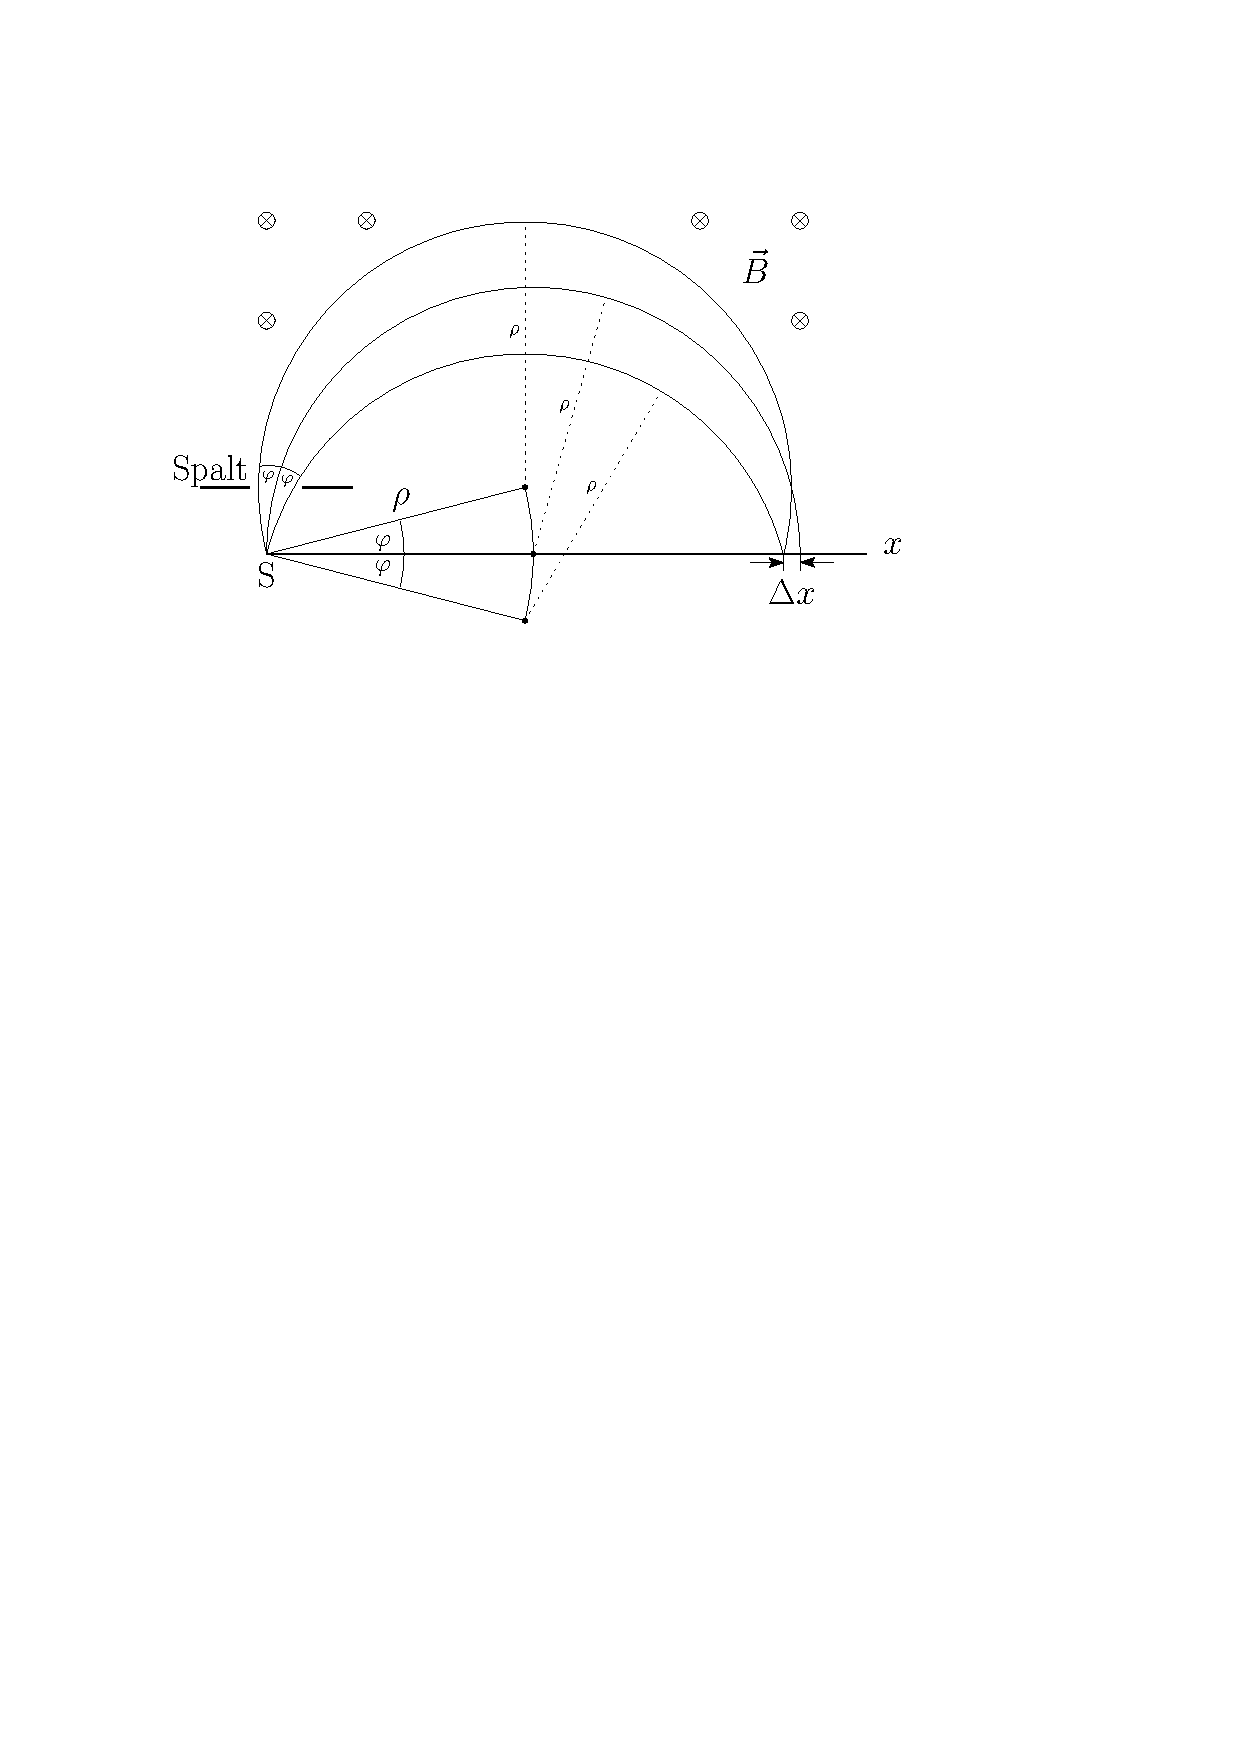
\includegraphics[width=0.8\textwidth]{./figures/semicircular_spectrometer.pdf}
	\caption{Halbkreisförmiges Spektrometer}
	\label{fig:semicirc_spectro}
\end{figure}
Ein halbkreisförmiges Spektrometer nutzt ein homogenes Magnetfeld senkrecht zur Flugrichtung der Elektronen um diese auf eine Kreisbahn zu lenken.
Nach Gleichung \eqref{eq:impuls_radius} ist das Produkt von Magnetfeld $B$ und Bahnradius $\rho$ charakteristisch für den Impuls des Elektrons.

Nachteil nur Fokussierung in der $\rho$-Ebene führt zu geringer Transmission.
Vorteil: einfache Konstruktion, Magnetfeld leicht zu messen, gut geeignet um große Spektralbereiche aufzunehmen (konstante Magnetfeldstärke)

\subsubsection{Doppelt-fokussierendes Spektrometer}
\begin{figure}[h]
	\centering
	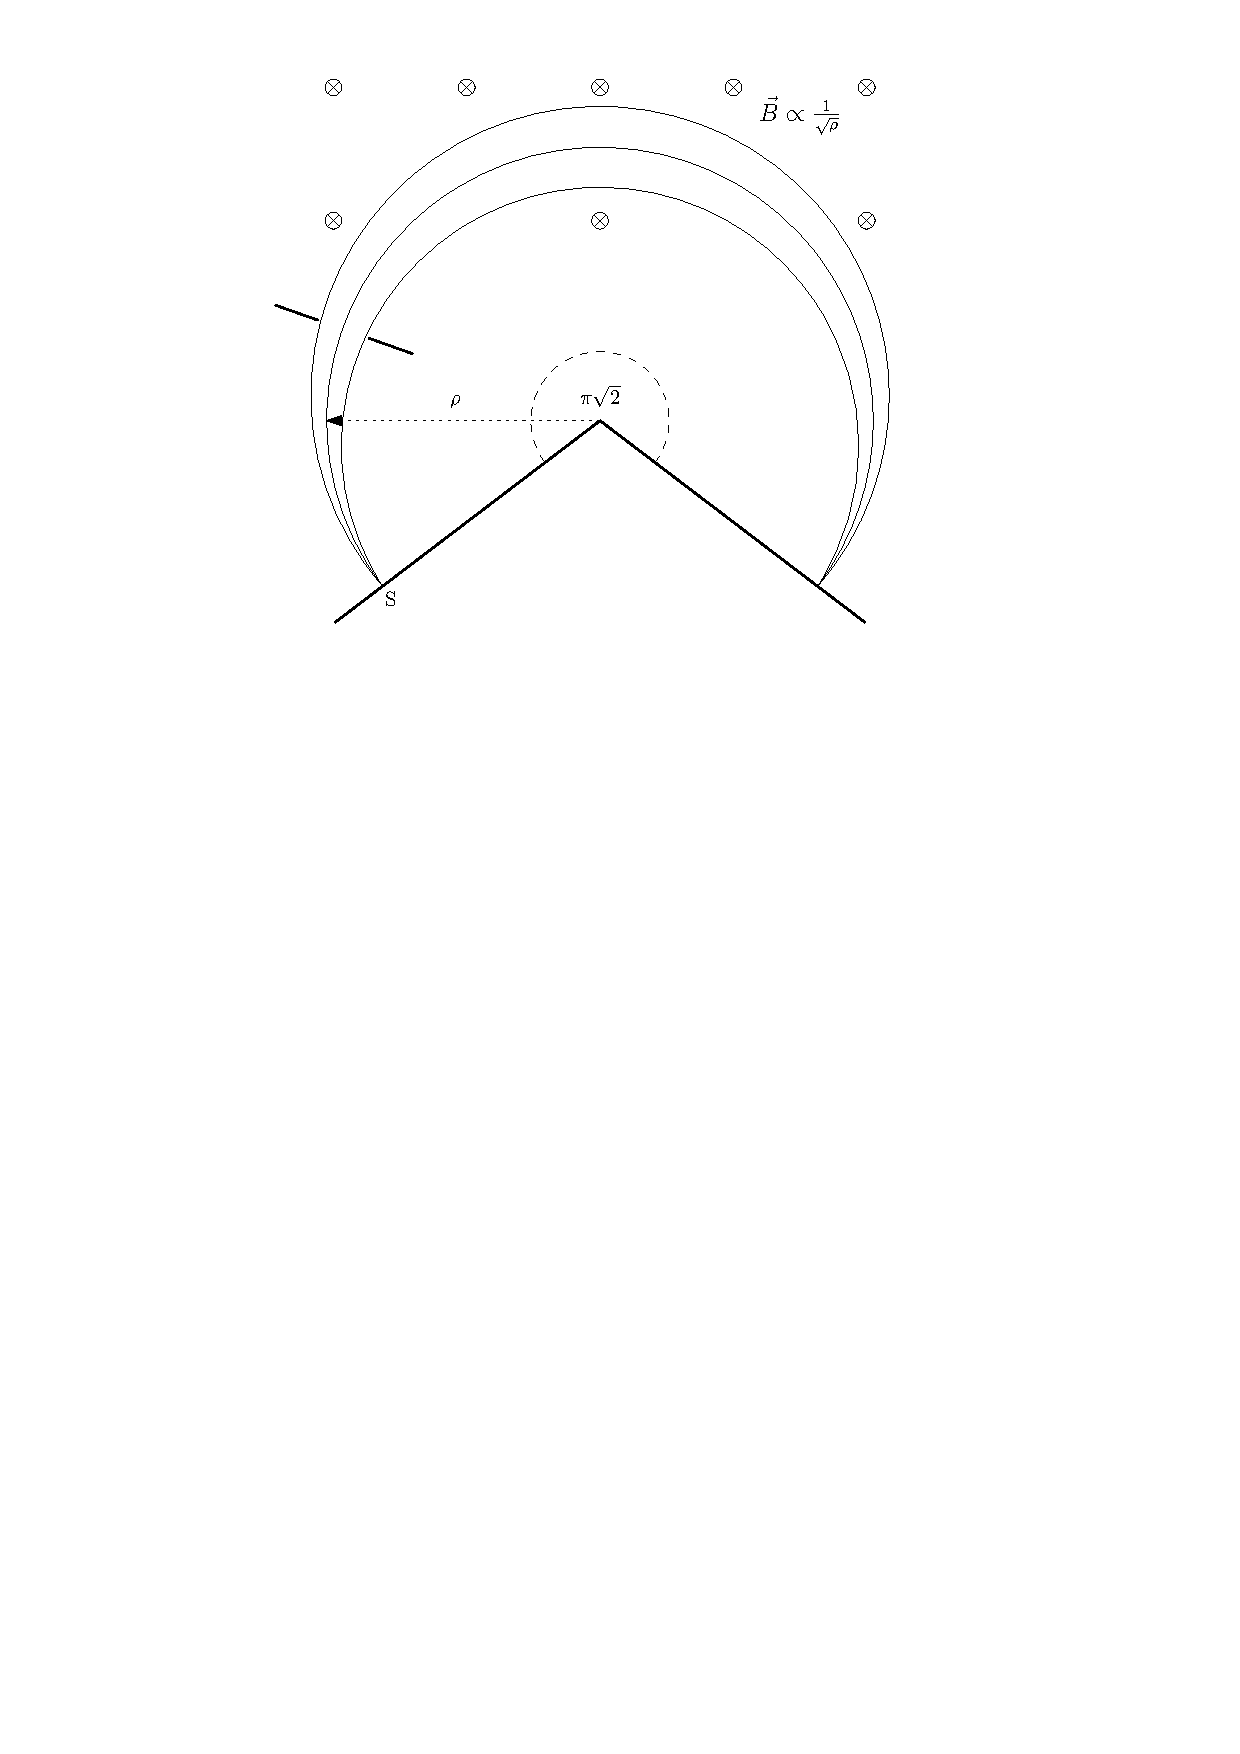
\includegraphics[width=0.8\textwidth]{./figures/pisqrt2_spectrometer.pdf}
	\caption{Doppelt-fokussierendes Spektrometer}
	\label{fig:pisqrt2_spectro}
\end{figure}
Betatron-Oszillationen ($\omega_0$: Elektronen Umlauffrequenz) (Zitat Hillert)
\begin{align}
	\omega_\rho = \omega_0 \sqrt{1-n} \qquad \omega_z = \omega_0 \sqrt{n}
\end{align}
mit dem Feldindex:
\begin{align}
	n = - \frac{\rho}{B_z(\rho)} \frac{\mathrm{d} B_z(\rho)}{\mathrm{d} \rho}
\end{align}
Während einer halben Periode der jeweiligen Betatronschwingung durchläuft das Elektron auf der Kreisbahn einen Winkel von:
\begin{align}
	\phi_\rho &= \omega_0 \cdot \frac{\pi}{\omega_\rho} & \phi_z &= \omega_0 \cdot \frac{\pi}{\omega_z}\\
	\phi_\rho &= \pi \left[ 1+ \frac{\rho_0 B^\prime(\rho_0)}{B(\rho_0)} \right]^{-\frac{1}{2}} & \phi_z &= \pi \left[ -\frac{\rho_0 B^\prime(\rho_0)}{B(\rho_0)} \right]^{-\frac{1}{2}} \label{eq:betatronwinkel}
\end{align}
ab, wobei $\rho_0$ den Radius der Sollbahn bezeichnet.
An Gleichung \eqref{eq:betatronwinkel} ließt man nach Quadrieren ab:
\begin{align}
	\frac{1}{\phi_\rho^2} + \frac{1}{\phi_z^2} = \frac{1}{\pi^2} \label{eq:betatronwinkelverhaeltnis}
\end{align}
Um eine stigmatische Abbildung zu erhalten (d.h. der Fokus der $\rho$- und $z$-Ebene liegen im selben Punkt) muss die Bedingung $\phi_\rho = \phi_z$ gestellt werden.
Damit folgt aus Gleichung \eqref{eq:betatronwinkelverhaeltnis} der gesamte Winkel der Elektronenbahn im Spektrometer.
Dieser ergibt sich zu $\phi = \pi \sqrt{2}$, weshalb das doppelt-fokussierende Spektrometer auch $\pi \sqrt{2}$-Spektrometer genannt wird.
Gleichzeitig folgt aus der gestellten Anforderung $\phi_\rho = \phi_z$ mit Gleichung \eqref{eq:betatronwinkel} die Bestimmungsgleichung für das magnetische Feld:
\begin{align}
	B^\prime(\rho) = - \frac{1}{2 \rho} B(\rho)
\end{align}
Mit der Randbedingung $B(\rho_0) = B_0$ folgt als allgemeine Lösung:
\begin{align}
	B(\rho) = B_0 \sqrt{\frac{\rho_0}{\rho}}
\end{align}
Der Vorteil gegenüber dem halbkreisförmigen Spektrometer liegt darin, dass das doppelt-fokussierende ebenfalls in der $z$-Ebene fokussierend wirkt und damit höhere Transmissionen möglich sind.

\subsection{Detektoren (?)}
\subsubsection{Halbleiterdetektoren}

\subsubsection{Hallsonde}

\subsubsection{Hysterese (?)}


\section{Durchführung und Auswertung}
Die ausführliche Durchführung ist der Versuchsanleitung \cite{anleitung} zu entnehmen.
Sollten Abweichungen bei der Durchführung auftreten, so werden diese im jeweiligen Unterkapitel dargestellt.

\subsection{Bestimmung der Offsetspannung der Hallsonde}
\label{ssec:offsetspannung}
\begin{wrapfigure}{o}{7.5cm}
	\centering
	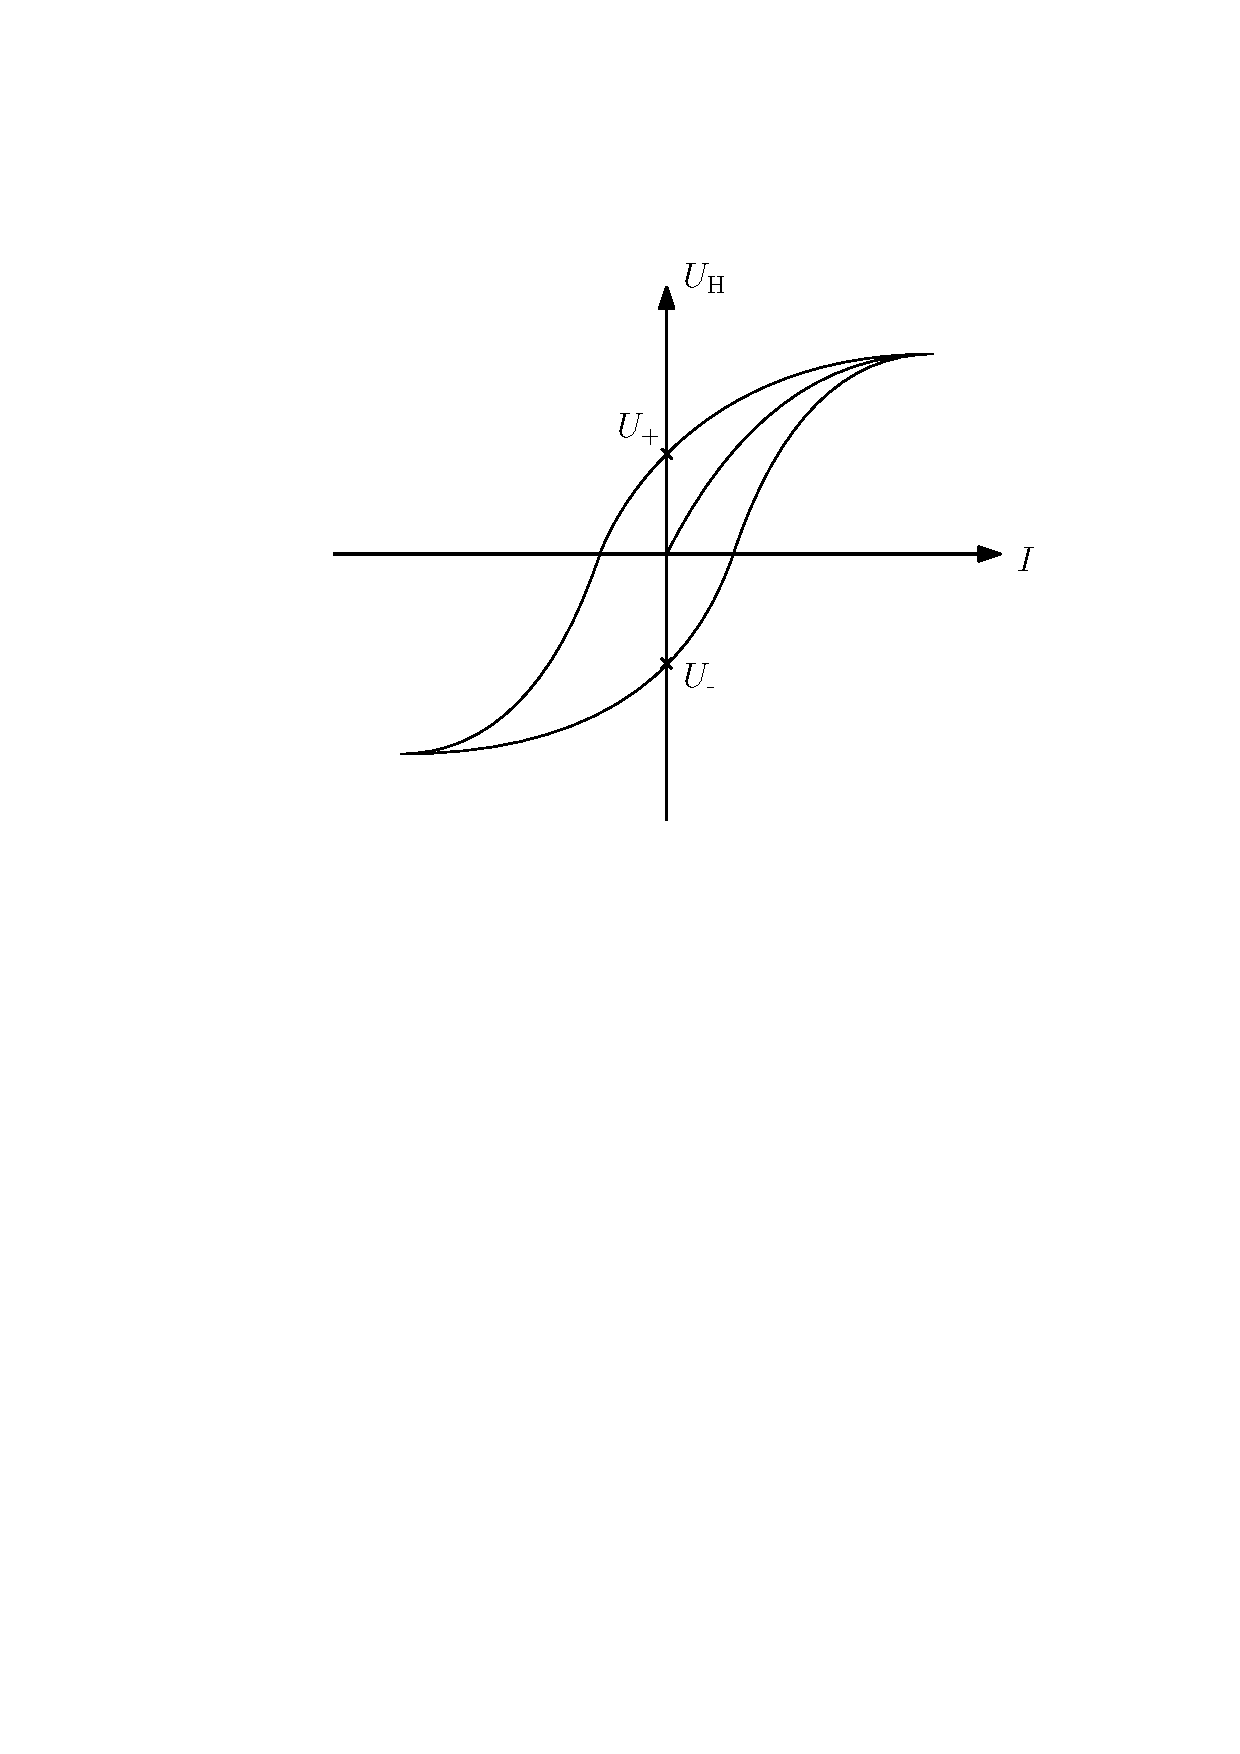
\includegraphics[width=0.5\textwidth]{./figures/hysterese.pdf}
	\caption{Skizzierte Hysteresekurve. Der tatsächliche Spannungswert für $I=\SI{0}{\ampere}$ ergibt sich aus Mittelung von $U_\text{+}$ und $U_\text{-}$.}
	\label{fig:hysterese}
\end{wrapfigure}
Zu Beginn des Versuchs wird zur Bestimmung der Offsetspannung das Spektrometer ohne Präparat evakuiert.
Die Messung des Magnetfelds des Spektrometers wird mit einer Hallsonde durchgeführt, die jedoch auch bei ausgeschaltetem Magnetfeld eine Spannung $\neq 0$ \si{\volt} anzeigt.
Um die tatsächliche Offsetspannung zu ermitteln, nutzt man die Hysterese des Magneten aus und misst für beide Stromrichtungen, die am Magneten angelegt werden die jeweiligen Remanenzfelder (als Hallspannung $U_\text{H}$) gemessen.
Bei jeder Messung wird das arithmetische Mittel (mit $U_0$ bezeichnet) von $U_\text{+}$ und $U_\text{-}$ berechnet und im Anschluss über alle $U_0$ wiederholt gemittelt, um einen guten Wert für die Offsetspannung $\overline{U_0}$ zu erhalten.
\begin{table}[h]
	\centering
	\begin{tabular}{SSSSSSS}
\toprule
{$U_+$ / \si{\skt}} & {$\Delta U_+$ / \si{\skt}} & {$U_-$ / \si{\skt}} & {$\Delta U_-$ / \si{\skt}} &  & {$U_0$ / \si{\skt}} & {$\Delta U_0$ / \si{\skt}} \\ \midrule
9.4 & 0.1    & 5.0 & 0.1    &  & 7.20   & 0.08   \\
9.4 & 0.1    & 5.0 & 0.1    &  & 7.20   & 0.08   \\
9.3 & 0.1    & 5.0 & 0.1    &  & 7.15   & 0.08   \\
9.3 & 0.1    & 5.0 & 0.1    &  & 7.15   & 0.08   \\
9.3 & 0.1    & 4.9 & 0.1    &  & 7.10   & 0.08   \\
9.3 & 0.1    & 5.0 & 0.1    &  & 7.15   & 0.08   \\ \midrule
    &        &     & {$\overline{U_0}$ / \si{\skt}:}    &  & 7.16   & 0.04   \\ \bottomrule
\end{tabular}
	\caption{Messwerte und Auswertung zur Bestimmung der Offsetspannung der Hallsonde. Die unterste Zeile ergibt sich aus Mittelung über alle $U_0$.}
	\label{tab:offset}
\end{table}
Der Fehler der Mittelung über $U_\text{+}$ und $U_\text{-}$ ergibt sich mit Gauß'scher Fehlerfortpflanzung aus
\begin{align}
	\Delta U_0 = \sqrt{(\Delta U_\text{+})^2 + (\Delta U_\text{-})^2}
\end{align}
Den im weiteren Verlauf benutzten Wert für die Offsetspannung $\overline{U_0}$ erhält man, indem über alle $U_0$ gemittelt wird. Da die Fehler auf $U_0$ gleich groß sind, ergibt sich für $\Delta\overline{U_0}$
\begin{align}
	\Delta\overline{U_0} = \frac{\Delta U_0}{\sqrt{6}}
\end{align}
und alle gemessenen Hallspannungen werden in der folgenden Auswertung um
\begin{align}
	\overline{U_0} = \SI{7.16 +- 0.03}{\skt}
	\label{hall_korrektur}
\end{align}
korrigiert.

\subsection{Kalibration des Spektrometers}
\label{ssec:kalibration}
Zur Kalibration des Spektrometers wird das Spektrum von \isotope[137]{Cs} bei Transmissionen von \SI{1}{\percent} und \SI{4}{\percent} vermessen.
Dazu wird das Präparat in das Spektrometer eingesetzt und die jeweilige Transmission eingestellt.
Nachdem die Messzeit festgelegt wurde, kann die Messung gestartet und die Zählrate an dem Impulszähler abgelesen werden.
Für die gleiche Messzeit und Transmission werden bei geändertem Magnetfeld Messungen wiederholt, aus denen sich ein Zerfallsspektrum ableiten lässt.
Von Interesse sind dabei die Konversionslinien des angeregten Isotops \isotope[137]{Ba}, welche zur Impulskalibrierung genutzt werden können.
Der angeregte Zustand von \isotope[137]{Ba} hat eine Zerfallsenergie von
\begin{align*}
	Q_\gamma = \SI{661,660}{\kilo\electronvolt}\text{.}
\end{align*}
Bei innerer Konversion überträgt sich diese Energie auf ein kernnahes Elektron, welches aus dem Atom gelöst wird.
Nach der Ionisation hat das Elektron eine kinetische Energie von
\begin{align}
	T = Q_\gamma - E_\mathrm{B} \text{,}
	\label{eq:kin_energie_konversion}
\end{align}
wobei $E_\mathrm{B}$ die Bindungsenergie des jeweiligen Elektrons im Atom bezeichnet.
Im Spektrum sind zwei Konversionslinien zu erkennen, welche der K- und L-Schale von Barium zuzuordnen sind.
Weiterhin muss beachtet werden, dass im Magnetfeld des Spektrometer eine Zeemanaufspaltung der Niveaus der L-Schale zu beobachten ist.
Zunächst soll die Konversionslinie des Elektrons der K-Schale mit der Bindungsenergie
\begin{align*}
E_\mathrm{K} = \SI{37,441}{\kilo\electronvolt}
\end{align*}
betrachtet werden.
Mit den Gleichungen \eqref{eq:b_rho} und \eqref{eq:kin_energie_konversion} kann der Impuls des Elektrons in der für die Spektroskopie üblichen Größe
\begin{align*}
	\left(B \rho \right)_\mathrm{K} = \SI{3381}{G.cm}
\end{align*}
angegeben werden.
\\
\\
Schließlich soll die Zeemanaufspaltung der L-Schale betrachtet werden, welche sich in drei diskrete Energieniveaus aufspaltet.
Für die Bindungsenergie der aufgespalteten Niveaus ist gegeben:
\begin{align*}
E_{\mathrm{L}_{\mathrm{I}}} = \SI{5,987}{\kilo\electronvolt} \quad
E_{\mathrm{L}_{\mathrm{II}}} = \SI{5,624}{\kilo\electronvolt} \quad
E_{\mathrm{L}_{\mathrm{III}}} = \SI{5,247}{\kilo\electronvolt}
\end{align*}
Da die Aufspaltung mit dem Spektroskop nicht auflösbar ist, muss eine sinnvolle Mittelung durchgeführt werden.
Dazu betrachtet man die Entartungsgrade der einzelnen Niveaus
\begin{align*}
g_{\mathrm{L}_{\mathrm{I}}} = \num{1} \quad
g_{\mathrm{L}_{\mathrm{II}}} = \num{2} \quad
g_{\mathrm{L}_{\mathrm{III}}} = \num{1}
\end{align*}
und führt eine dementsprechend gewichtete Mittelung durch:
\begin{align*}
E_\mathrm{L} = \frac{E_{\mathrm{L}_{\mathrm{I}}} + 2E_{\mathrm{L}_{\mathrm{II}}} + E_{\mathrm{L}_{\mathrm{III}}}}{4} \approx \SI{5,621}{\kilo\electronvolt}
\end{align*}
In Analogie zur K-Schale kann der Impuls des Elektrons berechnet werden:
\begin{align}
\left(B \rho \right)_\mathrm{L} = \SI{3500}{G.cm}
\end{align}

\subsubsection{Untergrundmessungen}
\label{sssec:untergrund1}
\begin{wraptable}{o}{0.5\textwidth}
	\centering
	\begin{tabular}{SSS}
\toprule
&{$N$ bei 1\% Transmission}  & {$N$ bei 4\% Transmission}   \\ \midrule
& 21     & 6         \\
& 24     & 8         \\
& 21     & 10        \\
& 21     & 8         \\
& 20     & 5         \\
& 21     & 13        \\
& 18     & 9         \\
& 15     & 3         \\
& 22     & 9         \\
& 18     & 9         \\\midrule
{Mittelwerte $N_0$:} & {\num{8+-2.8}} & {\num{20.1+-2.6}} \\ \bottomrule
\end{tabular}

	\caption{Untergrundmessung von \isotope[137]{Cs} bei 1\% und 4\% Transmission}
	\label{tab:untergrund_cs}
\end{wraptable}
Zur späteren Bereinigung der Messwerte werden vorher Untergrundmessungen durchgeführt.
Um möglichst hohe Zählraten zu erzielen wurde die Messzeit bei eingebautem Präparat bei 4\% Transmission auf \SI{40}{\second} eingestellt und für 1\% Transmission auf \SI{100}{\second} erhöht.
Durch eine nicht ideale Kalibration der Zähleinheit konnten jedoch nicht die in der Praktikumsanleitung empfohlene Zählraten erreicht werden.
Für den Untergrund des Caesium-Zerfalls bei beiden Transmissionseinstellungen sind die in Tabelle \ref{tab:untergrund_cs} notierten Werte für die Zählrate $N$ gemessen worden.
Die Messwerte wurden dabei in der untersten Zeile gemittelt und der Fehler aus der Standardabweichung berechnet.

\subsubsection{Spektrum von Caesium}
\label{sssec:spektrum_caesium}
Bei der Aufnahme des Spektrums wurde die Hallspannung $U_\mathrm{H}$ und die Anzahl der Ereignisse $N$ gemessen.
Dabei wird der Fehler der gemessenen Hallspannung aufgrund fehlender Kenntnis über das genaue Messverfahren auf
\begin{align*}
	\Delta U_\mathrm{H} = \SI{0.1}{\skt}
\end{align*}
festgelegt, was der letzten Stelle der Digitalanzeige entspricht.
Der Schätzwert für den Fehler der Ereigniszahl ergibt sich gemäß der Poisson-Verteilung (diese Annahme ist gültig, da die Zählraten poisson-verteilt sind) aus der Wurzel der Ereignisse:
\begin{align*}
	\Delta N = \sqrt{N}
\end{align*}
Zunächst muss die Hallspannung $U_\mathrm{H}$ um die in Abschnitt \ref{ssec:offsetspannung} ermittelte Offsetspannung $\overline{U_0}$ \eqref{hall_korrektur} bereinigt werden.
Die korrigierte Hallspannung erhält man durch:
\begin{align}
U_\mathrm{H}^\mathrm{korr.} = U_\mathrm{H} - \overline{U_0} \qquad
\Delta U_\mathrm{H}^\mathrm{korr.} = \sqrt{\Delta U_\mathrm{H}^2 + \Delta \overline{U_0}^2} \text{,}
\end{align}
wobei der Fehler aus der Gauß'schen Fehlerfortpflanzung folgt.
Für die Bereinigung der Zählraten mit den in Abschnitt \ref{sssec:untergrund1} gefundenen Werten für den Hintergrund gilt
\begin{align}
	N_\mathrm{korr.} = N - N_0 \qquad \Delta N_\mathrm{korr.} = \sqrt{\Delta N^2 + \Delta N_0^2}
\end{align}
wobei abermals die Gauß'sche Fehlerfortpflanzung für den Fehler angewendet wurde.
Weiterhin ist aufgrund der Dispersion des Spektrometers das gemessene Impulsintervall proportional zum anliegenden Magnetfeld.
Um eine vom Magnetfeld unabhängige Impulsverteilung zu erhalten, kann die Anzahl der um den Untergrund bereinigten Ereignisse durch eine zum Magnetfeld proportionale Größe dividiert werden.
Es liegt nahe die korrigierte Hallspannung $U_\mathrm{H}^\mathrm{korr.}$ zu diesem Zweck zu verwenden, sodass man die Impulsverteilung $n$ erhält:
\begin{align}
	n = \frac{N_\mathrm{korr.}}{U_\mathrm{H}^\mathrm{korr.}} \qquad \Delta n = \sqrt{\left( \frac{\Delta N_\mathrm{korr.}}{U_\mathrm{H}^\mathrm{korr.}}\right)^2 + \left( \frac{N_\mathrm{korr.} \cdot \Delta U_\mathrm{H}^\mathrm{korr.}}{ {U_\mathrm{H}^\mathrm{korr.}}^2 }\right)^2}
\end{align}
Trägt man die Impulsverteilung $n$ gegen die korrigierte Hallspannung $U_\mathrm{H}^\mathrm{korr.}$ auf, so erhält die Abbildung \ref{fig:ba_t4_grob}.
Dort sieht man eine Erhöhung der Zählrate bei ca. $U_\mathrm{H}^\mathrm{korr.} \approx \SI{150}{\skt}$, welche auf die Konversionslinien des angeregten Bariumkerns hindeutet.
Im folgenden Abschnitt sollen diese zur Impulskalibration genauer untersucht werden.
\begin{figure}[h]
	\centering
	% GNUPLOT: LaTeX picture with Postscript
\begingroup
  \makeatletter
  \providecommand\color[2][]{%
    \GenericError{(gnuplot) \space\space\space\@spaces}{%
      Package color not loaded in conjunction with
      terminal option `colourtext'%
    }{See the gnuplot documentation for explanation.%
    }{Either use 'blacktext' in gnuplot or load the package
      color.sty in LaTeX.}%
    \renewcommand\color[2][]{}%
  }%
  \providecommand\includegraphics[2][]{%
    \GenericError{(gnuplot) \space\space\space\@spaces}{%
      Package graphicx or graphics not loaded%
    }{See the gnuplot documentation for explanation.%
    }{The gnuplot epslatex terminal needs graphicx.sty or graphics.sty.}%
    \renewcommand\includegraphics[2][]{}%
  }%
  \providecommand\rotatebox[2]{#2}%
  \@ifundefined{ifGPcolor}{%
    \newif\ifGPcolor
    \GPcolortrue
  }{}%
  \@ifundefined{ifGPblacktext}{%
    \newif\ifGPblacktext
    \GPblacktexttrue
  }{}%
  % define a \g@addto@macro without @ in the name:
  \let\gplgaddtomacro\g@addto@macro
  % define empty templates for all commands taking text:
  \gdef\gplbacktext{}%
  \gdef\gplfronttext{}%
  \makeatother
  \ifGPblacktext
    % no textcolor at all
    \def\colorrgb#1{}%
    \def\colorgray#1{}%
  \else
    % gray or color?
    \ifGPcolor
      \def\colorrgb#1{\color[rgb]{#1}}%
      \def\colorgray#1{\color[gray]{#1}}%
      \expandafter\def\csname LTw\endcsname{\color{white}}%
      \expandafter\def\csname LTb\endcsname{\color{black}}%
      \expandafter\def\csname LTa\endcsname{\color{black}}%
      \expandafter\def\csname LT0\endcsname{\color[rgb]{1,0,0}}%
      \expandafter\def\csname LT1\endcsname{\color[rgb]{0,1,0}}%
      \expandafter\def\csname LT2\endcsname{\color[rgb]{0,0,1}}%
      \expandafter\def\csname LT3\endcsname{\color[rgb]{1,0,1}}%
      \expandafter\def\csname LT4\endcsname{\color[rgb]{0,1,1}}%
      \expandafter\def\csname LT5\endcsname{\color[rgb]{1,1,0}}%
      \expandafter\def\csname LT6\endcsname{\color[rgb]{0,0,0}}%
      \expandafter\def\csname LT7\endcsname{\color[rgb]{1,0.3,0}}%
      \expandafter\def\csname LT8\endcsname{\color[rgb]{0.5,0.5,0.5}}%
    \else
      % gray
      \def\colorrgb#1{\color{black}}%
      \def\colorgray#1{\color[gray]{#1}}%
      \expandafter\def\csname LTw\endcsname{\color{white}}%
      \expandafter\def\csname LTb\endcsname{\color{black}}%
      \expandafter\def\csname LTa\endcsname{\color{black}}%
      \expandafter\def\csname LT0\endcsname{\color{black}}%
      \expandafter\def\csname LT1\endcsname{\color{black}}%
      \expandafter\def\csname LT2\endcsname{\color{black}}%
      \expandafter\def\csname LT3\endcsname{\color{black}}%
      \expandafter\def\csname LT4\endcsname{\color{black}}%
      \expandafter\def\csname LT5\endcsname{\color{black}}%
      \expandafter\def\csname LT6\endcsname{\color{black}}%
      \expandafter\def\csname LT7\endcsname{\color{black}}%
      \expandafter\def\csname LT8\endcsname{\color{black}}%
    \fi
  \fi
    \setlength{\unitlength}{0.0500bp}%
    \ifx\gptboxheight\undefined%
      \newlength{\gptboxheight}%
      \newlength{\gptboxwidth}%
      \newsavebox{\gptboxtext}%
    \fi%
    \setlength{\fboxrule}{0.5pt}%
    \setlength{\fboxsep}{1pt}%
\begin{picture}(7200.00,5040.00)%
    \gplgaddtomacro\gplbacktext{%
      \csname LTb\endcsname%
      \put(946,704){\makebox(0,0)[r]{\strut{}$-0{,}5$}}%
      \csname LTb\endcsname%
      \put(946,1518){\makebox(0,0)[r]{\strut{}$0$}}%
      \csname LTb\endcsname%
      \put(946,2332){\makebox(0,0)[r]{\strut{}$0{,}5$}}%
      \csname LTb\endcsname%
      \put(946,3147){\makebox(0,0)[r]{\strut{}$1$}}%
      \csname LTb\endcsname%
      \put(946,3961){\makebox(0,0)[r]{\strut{}$1{,}5$}}%
      \csname LTb\endcsname%
      \put(946,4775){\makebox(0,0)[r]{\strut{}$2$}}%
      \csname LTb\endcsname%
      \put(1078,484){\makebox(0,0){\strut{}$0$}}%
      \csname LTb\endcsname%
      \put(1651,484){\makebox(0,0){\strut{}$20$}}%
      \csname LTb\endcsname%
      \put(2223,484){\makebox(0,0){\strut{}$40$}}%
      \csname LTb\endcsname%
      \put(2796,484){\makebox(0,0){\strut{}$60$}}%
      \csname LTb\endcsname%
      \put(3368,484){\makebox(0,0){\strut{}$80$}}%
      \csname LTb\endcsname%
      \put(3941,484){\makebox(0,0){\strut{}$100$}}%
      \csname LTb\endcsname%
      \put(4513,484){\makebox(0,0){\strut{}$120$}}%
      \csname LTb\endcsname%
      \put(5086,484){\makebox(0,0){\strut{}$140$}}%
      \csname LTb\endcsname%
      \put(5658,484){\makebox(0,0){\strut{}$160$}}%
      \csname LTb\endcsname%
      \put(6231,484){\makebox(0,0){\strut{}$180$}}%
      \csname LTb\endcsname%
      \put(6803,484){\makebox(0,0){\strut{}$200$}}%
    }%
    \gplgaddtomacro\gplfronttext{%
      \csname LTb\endcsname%
      \put(176,2739){\rotatebox{-270}{\makebox(0,0){\strut{}$n$}}}%
      \put(3940,154){\makebox(0,0){\strut{}$U_\mathrm{H}$ / \si{\skt}}}%
      \csname LTb\endcsname%
      \put(5816,4602){\makebox(0,0)[r]{\strut{}Messwerte}}%
    }%
    \gplbacktext
    \put(0,0){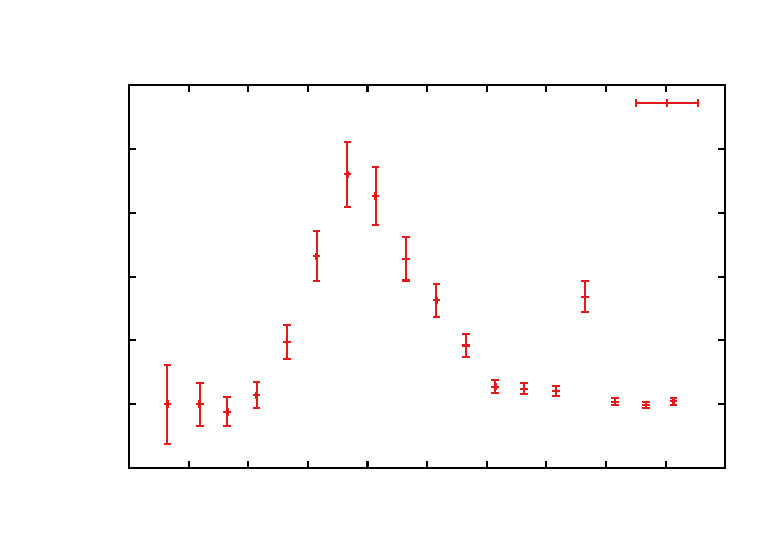
\includegraphics{./plots/barium_t4_grob}}%
    \gplfronttext
  \end{picture}%
\endgroup

	\caption{Spektrum von \isotope[137]{Cs} gemessen bei \SI{4}{\percent} Transmission mit einer Messdauer von \SI{40}{\second}. Sichtbar sind die Konversionslinien des angeregten \isotope[137]{Ba} Tochterkerns bei $U_\mathrm{H}^\mathrm{korr.} \approx \SI{150}{\skt}$}
	\label{fig:ba_t4_grob}
\end{figure}

\subsubsection{Impulskalibration}
\label{sssec:konversionslinien}
Zusätzlich zu der groben Aufnahme des Spektrums wurde der Bereich der Konversionslinien mit zwei verschiedenen Transmissionen $T = \SI{4}{\percent}$ (bei einer Messdauer von \SI{40}{\second}) und $T = \SI{1}{\percent}$ (bei einer Messdauer von \SI{100}{\second}) vermessen.
Die Messdaten und die daraus abgeleiteten Größen wurden in Tabellen \ref{tab:spektrum_ba4_fein} und \ref{tab:spektrum_ba1_fein} dargestellt, wobei die Berechnung der abgeleiteten Größen in Analogie zu Abschnitt \ref{sssec:spektrum_caesium} erfolgte.
\\
\\
Sichtbar sind die Konversionslinien der K- und L-Schale des angeregten Barium-Kerns, an welche mithilfe von \texttt{gnuplot} die Summe zweier Gaußfunktionen mit Offset angepasst wurde. Konkret lautet die Anpassungshypothese
\begin{align*}
	f(x) = \mathcal{G}_1(x) + \mathcal{G}_2(x) + b \text{,}
\end{align*}
wobei $\mathcal{G}$ die Gaußfunktion
\begin{align*}
	\mathcal{G}(x) = A \cdot \exp\left( - \frac{(x - \mu)^2}{2 \sigma^2}\right)
\end{align*}
mit dem Schwerpunkt $\mu$ und der Breite (Standardabweichung) $\sigma$ beschreibt.
\begin{figure}[h]
	\centering
	% GNUPLOT: LaTeX picture with Postscript
\begingroup
  \makeatletter
  \providecommand\color[2][]{%
    \GenericError{(gnuplot) \space\space\space\@spaces}{%
      Package color not loaded in conjunction with
      terminal option `colourtext'%
    }{See the gnuplot documentation for explanation.%
    }{Either use 'blacktext' in gnuplot or load the package
      color.sty in LaTeX.}%
    \renewcommand\color[2][]{}%
  }%
  \providecommand\includegraphics[2][]{%
    \GenericError{(gnuplot) \space\space\space\@spaces}{%
      Package graphicx or graphics not loaded%
    }{See the gnuplot documentation for explanation.%
    }{The gnuplot epslatex terminal needs graphicx.sty or graphics.sty.}%
    \renewcommand\includegraphics[2][]{}%
  }%
  \providecommand\rotatebox[2]{#2}%
  \@ifundefined{ifGPcolor}{%
    \newif\ifGPcolor
    \GPcolortrue
  }{}%
  \@ifundefined{ifGPblacktext}{%
    \newif\ifGPblacktext
    \GPblacktexttrue
  }{}%
  % define a \g@addto@macro without @ in the name:
  \let\gplgaddtomacro\g@addto@macro
  % define empty templates for all commands taking text:
  \gdef\gplbacktext{}%
  \gdef\gplfronttext{}%
  \makeatother
  \ifGPblacktext
    % no textcolor at all
    \def\colorrgb#1{}%
    \def\colorgray#1{}%
  \else
    % gray or color?
    \ifGPcolor
      \def\colorrgb#1{\color[rgb]{#1}}%
      \def\colorgray#1{\color[gray]{#1}}%
      \expandafter\def\csname LTw\endcsname{\color{white}}%
      \expandafter\def\csname LTb\endcsname{\color{black}}%
      \expandafter\def\csname LTa\endcsname{\color{black}}%
      \expandafter\def\csname LT0\endcsname{\color[rgb]{1,0,0}}%
      \expandafter\def\csname LT1\endcsname{\color[rgb]{0,1,0}}%
      \expandafter\def\csname LT2\endcsname{\color[rgb]{0,0,1}}%
      \expandafter\def\csname LT3\endcsname{\color[rgb]{1,0,1}}%
      \expandafter\def\csname LT4\endcsname{\color[rgb]{0,1,1}}%
      \expandafter\def\csname LT5\endcsname{\color[rgb]{1,1,0}}%
      \expandafter\def\csname LT6\endcsname{\color[rgb]{0,0,0}}%
      \expandafter\def\csname LT7\endcsname{\color[rgb]{1,0.3,0}}%
      \expandafter\def\csname LT8\endcsname{\color[rgb]{0.5,0.5,0.5}}%
    \else
      % gray
      \def\colorrgb#1{\color{black}}%
      \def\colorgray#1{\color[gray]{#1}}%
      \expandafter\def\csname LTw\endcsname{\color{white}}%
      \expandafter\def\csname LTb\endcsname{\color{black}}%
      \expandafter\def\csname LTa\endcsname{\color{black}}%
      \expandafter\def\csname LT0\endcsname{\color{black}}%
      \expandafter\def\csname LT1\endcsname{\color{black}}%
      \expandafter\def\csname LT2\endcsname{\color{black}}%
      \expandafter\def\csname LT3\endcsname{\color{black}}%
      \expandafter\def\csname LT4\endcsname{\color{black}}%
      \expandafter\def\csname LT5\endcsname{\color{black}}%
      \expandafter\def\csname LT6\endcsname{\color{black}}%
      \expandafter\def\csname LT7\endcsname{\color{black}}%
      \expandafter\def\csname LT8\endcsname{\color{black}}%
    \fi
  \fi
    \setlength{\unitlength}{0.0500bp}%
    \ifx\gptboxheight\undefined%
      \newlength{\gptboxheight}%
      \newlength{\gptboxwidth}%
      \newsavebox{\gptboxtext}%
    \fi%
    \setlength{\fboxrule}{0.5pt}%
    \setlength{\fboxsep}{1pt}%
\begin{picture}(7200.00,5040.00)%
    \gplgaddtomacro\gplbacktext{%
      \csname LTb\endcsname%
      \put(814,704){\makebox(0,0)[r]{\strut{}$0$}}%
      \put(814,1286){\makebox(0,0)[r]{\strut{}$0{,}2$}}%
      \put(814,1867){\makebox(0,0)[r]{\strut{}$0{,}4$}}%
      \put(814,2449){\makebox(0,0)[r]{\strut{}$0{,}6$}}%
      \put(814,3030){\makebox(0,0)[r]{\strut{}$0{,}8$}}%
      \put(814,3612){\makebox(0,0)[r]{\strut{}$1$}}%
      \put(814,4193){\makebox(0,0)[r]{\strut{}$1{,}2$}}%
      \put(814,4775){\makebox(0,0)[r]{\strut{}$1{,}4$}}%
      \put(1434,484){\makebox(0,0){\strut{}$148$}}%
      \put(2410,484){\makebox(0,0){\strut{}$150$}}%
      \put(3386,484){\makebox(0,0){\strut{}$152$}}%
      \put(4363,484){\makebox(0,0){\strut{}$154$}}%
      \put(5339,484){\makebox(0,0){\strut{}$156$}}%
      \put(6315,484){\makebox(0,0){\strut{}$158$}}%
    }%
    \gplgaddtomacro\gplfronttext{%
      \csname LTb\endcsname%
      \put(176,2739){\rotatebox{-270}{\makebox(0,0){\strut{}$n$}}}%
      \put(3874,154){\makebox(0,0){\strut{}$U_\mathrm{H}$ / \si{\skt}}}%
      \csname LTb\endcsname%
      \put(5816,4602){\makebox(0,0)[r]{\strut{}Messwerte}}%
      \csname LTb\endcsname%
      \put(5816,4382){\makebox(0,0)[r]{\strut{}g(x)}}%
    }%
    \gplbacktext
    \put(0,0){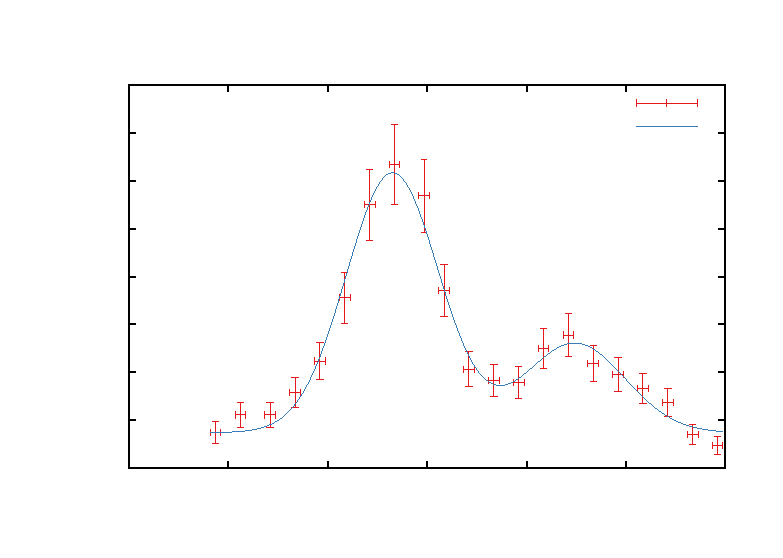
\includegraphics{./plots/barium_t4_fein}}%
    \gplfronttext
  \end{picture}%
\endgroup

	\caption{Bereich der K- und L-Konversionslinien des angeregten \isotope[137]{Ba} Tochterkerns im Zerfall von \isotope[137]{Cs} bei \SI{4}{\percent} Transmission und einer Messdauer von \SI{40}{\second}. An die Datenpunkte wurde eine Summe von zwei Gaußfunktionen mit konstantem Versatz angepasst.}
	\label{fig:ba_t4_fein}
\end{figure}
\begin{figure}[h]
	\centering
	% GNUPLOT: LaTeX picture with Postscript
\begingroup
  \makeatletter
  \providecommand\color[2][]{%
    \GenericError{(gnuplot) \space\space\space\@spaces}{%
      Package color not loaded in conjunction with
      terminal option `colourtext'%
    }{See the gnuplot documentation for explanation.%
    }{Either use 'blacktext' in gnuplot or load the package
      color.sty in LaTeX.}%
    \renewcommand\color[2][]{}%
  }%
  \providecommand\includegraphics[2][]{%
    \GenericError{(gnuplot) \space\space\space\@spaces}{%
      Package graphicx or graphics not loaded%
    }{See the gnuplot documentation for explanation.%
    }{The gnuplot epslatex terminal needs graphicx.sty or graphics.sty.}%
    \renewcommand\includegraphics[2][]{}%
  }%
  \providecommand\rotatebox[2]{#2}%
  \@ifundefined{ifGPcolor}{%
    \newif\ifGPcolor
    \GPcolortrue
  }{}%
  \@ifundefined{ifGPblacktext}{%
    \newif\ifGPblacktext
    \GPblacktexttrue
  }{}%
  % define a \g@addto@macro without @ in the name:
  \let\gplgaddtomacro\g@addto@macro
  % define empty templates for all commands taking text:
  \gdef\gplbacktext{}%
  \gdef\gplfronttext{}%
  \makeatother
  \ifGPblacktext
    % no textcolor at all
    \def\colorrgb#1{}%
    \def\colorgray#1{}%
  \else
    % gray or color?
    \ifGPcolor
      \def\colorrgb#1{\color[rgb]{#1}}%
      \def\colorgray#1{\color[gray]{#1}}%
      \expandafter\def\csname LTw\endcsname{\color{white}}%
      \expandafter\def\csname LTb\endcsname{\color{black}}%
      \expandafter\def\csname LTa\endcsname{\color{black}}%
      \expandafter\def\csname LT0\endcsname{\color[rgb]{1,0,0}}%
      \expandafter\def\csname LT1\endcsname{\color[rgb]{0,1,0}}%
      \expandafter\def\csname LT2\endcsname{\color[rgb]{0,0,1}}%
      \expandafter\def\csname LT3\endcsname{\color[rgb]{1,0,1}}%
      \expandafter\def\csname LT4\endcsname{\color[rgb]{0,1,1}}%
      \expandafter\def\csname LT5\endcsname{\color[rgb]{1,1,0}}%
      \expandafter\def\csname LT6\endcsname{\color[rgb]{0,0,0}}%
      \expandafter\def\csname LT7\endcsname{\color[rgb]{1,0.3,0}}%
      \expandafter\def\csname LT8\endcsname{\color[rgb]{0.5,0.5,0.5}}%
    \else
      % gray
      \def\colorrgb#1{\color{black}}%
      \def\colorgray#1{\color[gray]{#1}}%
      \expandafter\def\csname LTw\endcsname{\color{white}}%
      \expandafter\def\csname LTb\endcsname{\color{black}}%
      \expandafter\def\csname LTa\endcsname{\color{black}}%
      \expandafter\def\csname LT0\endcsname{\color{black}}%
      \expandafter\def\csname LT1\endcsname{\color{black}}%
      \expandafter\def\csname LT2\endcsname{\color{black}}%
      \expandafter\def\csname LT3\endcsname{\color{black}}%
      \expandafter\def\csname LT4\endcsname{\color{black}}%
      \expandafter\def\csname LT5\endcsname{\color{black}}%
      \expandafter\def\csname LT6\endcsname{\color{black}}%
      \expandafter\def\csname LT7\endcsname{\color{black}}%
      \expandafter\def\csname LT8\endcsname{\color{black}}%
    \fi
  \fi
    \setlength{\unitlength}{0.0500bp}%
    \ifx\gptboxheight\undefined%
      \newlength{\gptboxheight}%
      \newlength{\gptboxwidth}%
      \newsavebox{\gptboxtext}%
    \fi%
    \setlength{\fboxrule}{0.5pt}%
    \setlength{\fboxsep}{1pt}%
\begin{picture}(7200.00,5040.00)%
    \gplgaddtomacro\gplbacktext{%
      \csname LTb\endcsname%
      \put(814,704){\makebox(0,0)[r]{\strut{}0{,}0}}%
      \csname LTb\endcsname%
      \put(814,1286){\makebox(0,0)[r]{\strut{}0{,}2}}%
      \csname LTb\endcsname%
      \put(814,1867){\makebox(0,0)[r]{\strut{}0{,}4}}%
      \csname LTb\endcsname%
      \put(814,2449){\makebox(0,0)[r]{\strut{}0{,}6}}%
      \csname LTb\endcsname%
      \put(814,3030){\makebox(0,0)[r]{\strut{}0{,}8}}%
      \csname LTb\endcsname%
      \put(814,3612){\makebox(0,0)[r]{\strut{}1{,}0}}%
      \csname LTb\endcsname%
      \put(814,4193){\makebox(0,0)[r]{\strut{}1{,}2}}%
      \csname LTb\endcsname%
      \put(814,4775){\makebox(0,0)[r]{\strut{}1{,}4}}%
      \csname LTb\endcsname%
      \put(946,484){\makebox(0,0){\strut{}$146$}}%
      \csname LTb\endcsname%
      \put(1783,484){\makebox(0,0){\strut{}$148$}}%
      \csname LTb\endcsname%
      \put(2619,484){\makebox(0,0){\strut{}$150$}}%
      \csname LTb\endcsname%
      \put(3456,484){\makebox(0,0){\strut{}$152$}}%
      \csname LTb\endcsname%
      \put(4293,484){\makebox(0,0){\strut{}$154$}}%
      \csname LTb\endcsname%
      \put(5130,484){\makebox(0,0){\strut{}$156$}}%
      \csname LTb\endcsname%
      \put(5966,484){\makebox(0,0){\strut{}$158$}}%
      \csname LTb\endcsname%
      \put(6803,484){\makebox(0,0){\strut{}$160$}}%
    }%
    \gplgaddtomacro\gplfronttext{%
      \csname LTb\endcsname%
      \put(176,2739){\rotatebox{-270}{\makebox(0,0){\strut{}$n$}}}%
      \put(3874,154){\makebox(0,0){\strut{}$ U_\mathrm{H}^\mathrm{korr.}$ / \si{\skt}}}%
      \csname LTb\endcsname%
      \put(5816,4602){\makebox(0,0)[r]{\strut{}Messwerte}}%
      \csname LTb\endcsname%
      \put(5816,4382){\makebox(0,0)[r]{\strut{}Anpassung}}%
    }%
    \gplbacktext
    \put(0,0){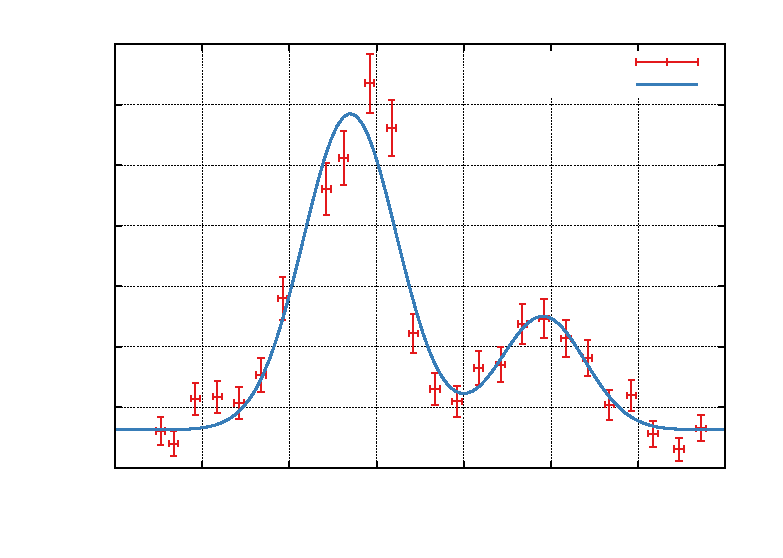
\includegraphics{./plots/barium_t1_fein}}%
    \gplfronttext
  \end{picture}%
\endgroup

	\caption{Bereich der K- und L-Konversionslinien des angeregten \isotope[137]{Ba} Tochterkerns im Zerfall von \isotope[137]{Cs} bei \SI{1}{\percent} Transmission und einer Messdauer von \SI{100}{\second}. An die Datenpunkte wurde eine Summe von zwei Gaußfunktionen mit konstantem Versatz angepasst.}
	\label{fig:ba_t1_fein}
\end{figure}
Die mit \texttt{gnuplot} gefundenen Werte für die Anpassungsparameter $\mu$ und $\sigma$ (die einer Spannung in Skalenteilen entsprechen) wurden für die jeweiligen Schalen und Transmissionen in Tabelle \ref{tab:fitergebnisse_ba} festgehalten.
Wie in der Darstellung ersichtlich ist die Anpassung für die Messwerte des bei \SI{1}{\percent} Transmission vor allem für die K-Schale nicht gut gelungen.
Man sieht eine deutliche Abweichung der Messwerte von einer Gaußfunktion, jedoch liefert die Anpassung der Schwerpunkte sinnvolle Werte, so dass diese für die Auswertung verwendet werden.
\begin{table}[h]
	\centering
	\begin{tabular}{SSSSS}
\toprule
{Linie}     & {$U_\mu$ / Skt} & {$\Delta U_\mu$ / Skt} & {$U_\sigma$ / Skt} & {$\Delta U_\sigma$ Skt} \\ \midrule
{K bei 4\%} & 151.34    & 0.06          & 0.92         & 0.06          \\
{L bei 4\%} & 154.96    & 0.14          & 1.00         & 0.16          \\
{K bei 1\%} & 151.40    & 0.10          & 1.08         & 0.10          \\
{L bei 1\%} & 155.82    & 0.18          & 0.98         & 0.14          \\ \bottomrule
\end{tabular}
	\caption{Ergebnisse der Anpassung für die Schwerpunkte der Konversionslinien von \isotope[137]{Ba} bei 1\% und 4\% Transmission.}
	\label{tab:fitergebnisse_ba}
\end{table}
Mit den angepassten Linienschwerpunkten kann nun die Impulskalibration durchgeführt werden.
Dazu wurden in Abschnitt \ref{ssec:kalibration} bereits die mit den Linien korrespondierenden $(B \rho)$-Werte berechnet.
Trägt man nun die Schwerpunkte der Linien $U_\mathrm{H}$ gegen den berechneten $(B \rho)$-Wert auf, so erhält man eine Ursprungsgerade mit der Steigung $m$.
Diese Form der Darstellung wurde gewählt, da bei der Anpassung einer Ursprungsgeraden mit \texttt{gnuplot} nur $y$-Fehler berücksichtigt werden können.
\begin{figure}[h]
	\centering
	% GNUPLOT: LaTeX picture with Postscript
\begingroup
  \makeatletter
  \providecommand\color[2][]{%
    \GenericError{(gnuplot) \space\space\space\@spaces}{%
      Package color not loaded in conjunction with
      terminal option `colourtext'%
    }{See the gnuplot documentation for explanation.%
    }{Either use 'blacktext' in gnuplot or load the package
      color.sty in LaTeX.}%
    \renewcommand\color[2][]{}%
  }%
  \providecommand\includegraphics[2][]{%
    \GenericError{(gnuplot) \space\space\space\@spaces}{%
      Package graphicx or graphics not loaded%
    }{See the gnuplot documentation for explanation.%
    }{The gnuplot epslatex terminal needs graphicx.sty or graphics.sty.}%
    \renewcommand\includegraphics[2][]{}%
  }%
  \providecommand\rotatebox[2]{#2}%
  \@ifundefined{ifGPcolor}{%
    \newif\ifGPcolor
    \GPcolortrue
  }{}%
  \@ifundefined{ifGPblacktext}{%
    \newif\ifGPblacktext
    \GPblacktexttrue
  }{}%
  % define a \g@addto@macro without @ in the name:
  \let\gplgaddtomacro\g@addto@macro
  % define empty templates for all commands taking text:
  \gdef\gplbacktext{}%
  \gdef\gplfronttext{}%
  \makeatother
  \ifGPblacktext
    % no textcolor at all
    \def\colorrgb#1{}%
    \def\colorgray#1{}%
  \else
    % gray or color?
    \ifGPcolor
      \def\colorrgb#1{\color[rgb]{#1}}%
      \def\colorgray#1{\color[gray]{#1}}%
      \expandafter\def\csname LTw\endcsname{\color{white}}%
      \expandafter\def\csname LTb\endcsname{\color{black}}%
      \expandafter\def\csname LTa\endcsname{\color{black}}%
      \expandafter\def\csname LT0\endcsname{\color[rgb]{1,0,0}}%
      \expandafter\def\csname LT1\endcsname{\color[rgb]{0,1,0}}%
      \expandafter\def\csname LT2\endcsname{\color[rgb]{0,0,1}}%
      \expandafter\def\csname LT3\endcsname{\color[rgb]{1,0,1}}%
      \expandafter\def\csname LT4\endcsname{\color[rgb]{0,1,1}}%
      \expandafter\def\csname LT5\endcsname{\color[rgb]{1,1,0}}%
      \expandafter\def\csname LT6\endcsname{\color[rgb]{0,0,0}}%
      \expandafter\def\csname LT7\endcsname{\color[rgb]{1,0.3,0}}%
      \expandafter\def\csname LT8\endcsname{\color[rgb]{0.5,0.5,0.5}}%
    \else
      % gray
      \def\colorrgb#1{\color{black}}%
      \def\colorgray#1{\color[gray]{#1}}%
      \expandafter\def\csname LTw\endcsname{\color{white}}%
      \expandafter\def\csname LTb\endcsname{\color{black}}%
      \expandafter\def\csname LTa\endcsname{\color{black}}%
      \expandafter\def\csname LT0\endcsname{\color{black}}%
      \expandafter\def\csname LT1\endcsname{\color{black}}%
      \expandafter\def\csname LT2\endcsname{\color{black}}%
      \expandafter\def\csname LT3\endcsname{\color{black}}%
      \expandafter\def\csname LT4\endcsname{\color{black}}%
      \expandafter\def\csname LT5\endcsname{\color{black}}%
      \expandafter\def\csname LT6\endcsname{\color{black}}%
      \expandafter\def\csname LT7\endcsname{\color{black}}%
      \expandafter\def\csname LT8\endcsname{\color{black}}%
    \fi
  \fi
    \setlength{\unitlength}{0.0500bp}%
    \ifx\gptboxheight\undefined%
      \newlength{\gptboxheight}%
      \newlength{\gptboxwidth}%
      \newsavebox{\gptboxtext}%
    \fi%
    \setlength{\fboxrule}{0.5pt}%
    \setlength{\fboxsep}{1pt}%
\begin{picture}(7200.00,5040.00)%
    \gplgaddtomacro\gplbacktext{%
      \csname LTb\endcsname%
      \put(814,704){\makebox(0,0)[r]{\strut{}$0$}}%
      \csname LTb\endcsname%
      \put(814,1156){\makebox(0,0)[r]{\strut{}$20$}}%
      \csname LTb\endcsname%
      \put(814,1609){\makebox(0,0)[r]{\strut{}$40$}}%
      \csname LTb\endcsname%
      \put(814,2061){\makebox(0,0)[r]{\strut{}$60$}}%
      \csname LTb\endcsname%
      \put(814,2513){\makebox(0,0)[r]{\strut{}$80$}}%
      \csname LTb\endcsname%
      \put(814,2966){\makebox(0,0)[r]{\strut{}$100$}}%
      \csname LTb\endcsname%
      \put(814,3418){\makebox(0,0)[r]{\strut{}$120$}}%
      \csname LTb\endcsname%
      \put(814,3870){\makebox(0,0)[r]{\strut{}$140$}}%
      \csname LTb\endcsname%
      \put(814,4323){\makebox(0,0)[r]{\strut{}$160$}}%
      \csname LTb\endcsname%
      \put(814,4775){\makebox(0,0)[r]{\strut{}$180$}}%
      \csname LTb\endcsname%
      \put(946,484){\makebox(0,0){\strut{}$0$}}%
      \csname LTb\endcsname%
      \put(1678,484){\makebox(0,0){\strut{}$500$}}%
      \csname LTb\endcsname%
      \put(2410,484){\makebox(0,0){\strut{}$1000$}}%
      \csname LTb\endcsname%
      \put(3142,484){\makebox(0,0){\strut{}$1500$}}%
      \csname LTb\endcsname%
      \put(3875,484){\makebox(0,0){\strut{}$2000$}}%
      \csname LTb\endcsname%
      \put(4607,484){\makebox(0,0){\strut{}$2500$}}%
      \csname LTb\endcsname%
      \put(5339,484){\makebox(0,0){\strut{}$3000$}}%
      \csname LTb\endcsname%
      \put(6071,484){\makebox(0,0){\strut{}$3500$}}%
      \csname LTb\endcsname%
      \put(6803,484){\makebox(0,0){\strut{}$4000$}}%
    }%
    \gplgaddtomacro\gplfronttext{%
      \csname LTb\endcsname%
      \put(176,2739){\rotatebox{-270}{\makebox(0,0){\strut{}$U_H$ / \si{\skt}}}}%
      \put(3874,154){\makebox(0,0){\strut{}$B \rho$ / \si{G.cm}}}%
      \csname LTb\endcsname%
      \put(5816,4602){\makebox(0,0)[r]{\strut{}Messwerte}}%
      \csname LTb\endcsname%
      \put(5816,4382){\makebox(0,0)[r]{\strut{}f(x)}}%
    }%
    \gplbacktext
    \put(0,0){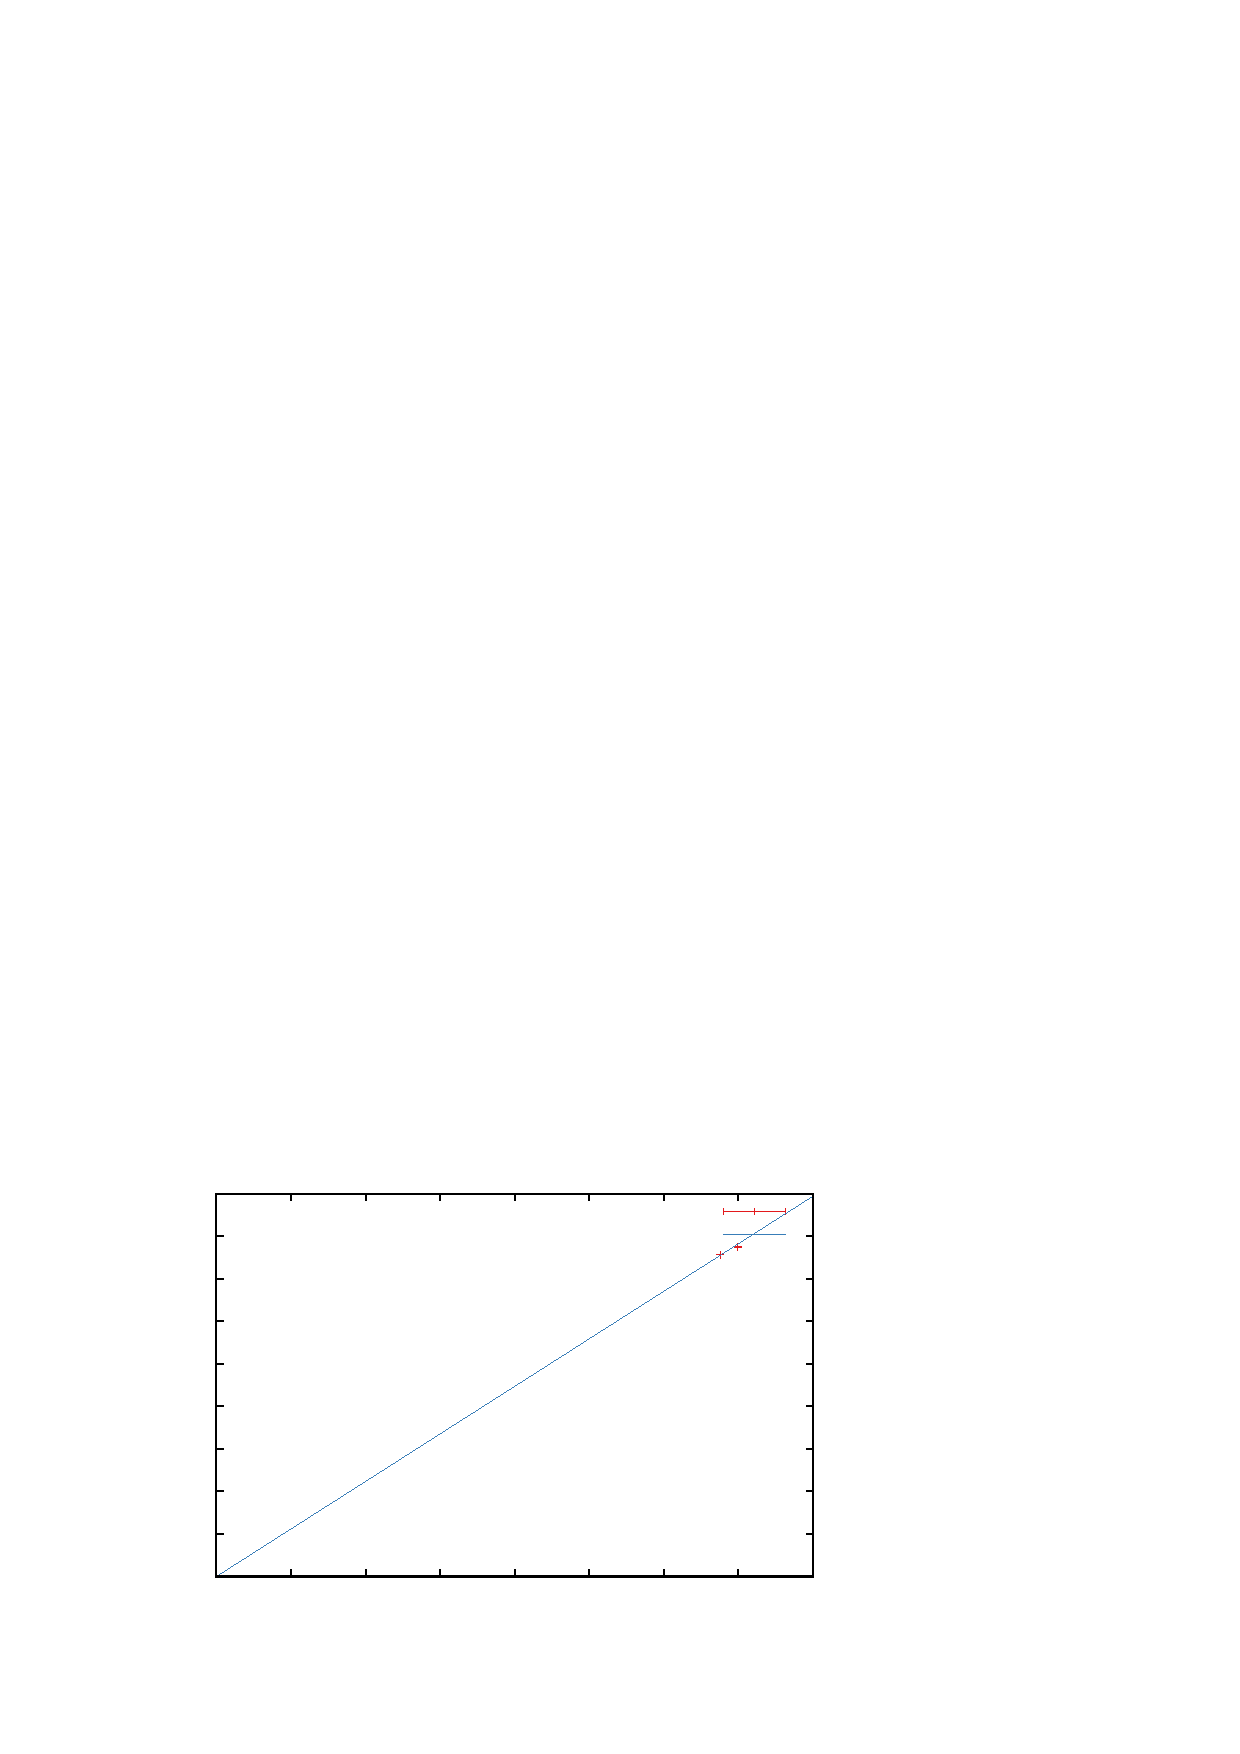
\includegraphics{./plots/kalibration}}%
    \gplfronttext
  \end{picture}%
\endgroup

	\caption{Anpassung der Kalibrationsgeraden an die gefundenen Linienschwerpunkte $U_\mathrm{H}$ und dem theoretisch berechneten $(B \rho)$-Wert der jeweiligen Linie bei beiden Transmissionen \num{1} und \SI{4}{\percent}. (FIXME)}
	\label{fig:kalibration}
\end{figure}
In Abbildung \ref{fig:kalibration} wurde die Anpassung der Ursprungsgerade  an die Kalibrationsdaten durchgeführt.
Es ergibt sich die Steigung:
\begin{align}
	m = \SI{0.0447 +- 0.0001}{\skt\per \gauss \per \centi\metre}
\end{align}
Aus der Steigung $m$ kann nun die Proportionalitätskonstante $\lambda$
\begin{align}
	B \rho = \lambda \cdot U_\mathrm{H}^\mathrm{korr.}
\end{align}
berechnet werden.
Dazu reicht die Bildung des Kehrwertes
\begin{align}
	\lambda = \frac{1}{m} \qquad \Delta \lambda = \frac{\Delta m}{m^2}
\end{align}
so dass man schlussendlich erhält:
\begin{align}
	\lambda = \SI{22.37 +- 0.05}{G.cm\per\skt}
\end{align}

\subsubsection{Auflösungsvermögen des Spektrometers}
Im Folgenden soll das Auflösungsvermögen des Spektrometers bei verschiedenen Transmissionen bestimmt werden.
Die für das Auflösungsvermögen relevante Größe ist dabei die relative Linienbreite $R$ aus Gleichung \eqref{eq:rel_linienbreite}.
Zur Berechnung wird die Halbwertsbreite sowie der Schwerpunkt der jeweiligen Linie benötigt.
Der Schwerpunkt $\mu$ der Linie ist direkt aus der Anpassung \ref{tab:fitergebnisse_ba} der Gaußfunktionen an die Linien abzulesen, lediglich bei der Bestimmung der Halbwertsbreite muss eine weitere Berechnung erfolgen, da nur die Standardabweichung der Gaußfunktion zur Verfügung steht.
\begin{align}
	\mathrm{FWHM} = 2 \sqrt{2\ln(2)} \cdot \sigma
\end{align}
Aufgrund des linearen Zusammenhangs zwischen Hallspannung $U_\mathrm{H}$ und Elektronenimpuls $(B \rho)$ kann auf die Umrechnung verzichtet werden, sodass gilt:
\begin{align*}
	R = \frac{\Delta (B \rho)}{B \rho} = \frac{\Delta U_\mathrm{H}^\mathrm{korr.}}{U_\mathrm{H}^\mathrm{korr.}}
\end{align*}
Bei diesen Berechnungen muss beachtet werden, dass mit $\Delta$ bezeichnete Größen in diesem Zusammenhang keinen Fehler angeben, sondern die jeweiligen Halbwertsbreiten darstellen.

\begin{table}[h]
	\centering
	\begin{tabular}{cSSSl}
\toprule
Linie  & {$R$}      & ${\Delta R}$     & \\
\midrule
K bei 4\% & 0.0140 & 0.0009 & \multirow{2}{*}{$\overline{R}_{4\%} = \SI{0.0142 +- 0.0008}{}$} \\
L bei 4\% & 0.0152 & 0.0023 &                    \\
K bei 1\% & 0.0167 & 0.0014 & \multirow{2}{*}{$\overline{R}_{1\%} = \SI{0.0160 +- 0.0011}{}$} \\
L bei 1\% & 0.0146 & 0.0020 &                    \\
%\cmidrule(r){1-4}
\bottomrule
\end{tabular}
	\caption{Auflösungsvermögen ($\Delta R$ bezeichnet hier wieder den Fehler)}
	\label{tab:aufloesungsvermoegen}
\end{table}

\subsection{Bestimmung der Zerfallsenergie}

\subsubsection{Spektrum von Thallium}
\begin{wraptable}{o}{4.7cm}
	\centering
	\begin{tabular}{c}
\toprule
{$N$} \\
\midrule
 45   \\
 45   \\
 48   \\
 48   \\
 51   \\
 55   \\
 44   \\
 39   \\
 54   \\
 41   \\
\midrule
{Mittelwert $N_0$} \\
\num{47 +- 5.2} \\
\bottomrule
\end{tabular}

	\caption{Untergrundmessung von \isotope[204]{Tl} mit einer Messdauer von \SI{100}{\second} bei \SI{4}{\percent} Transmission.}
	\label{tab:untergrund_tl}
\end{wraptable}
Bei der Vermessung des Spektrums von Thallium wurde analog zu Abschnitt \ref{sssec:spektrum_caesium} vorgegangen mit der Ausnahme, dass die Hallspannungen mit der in \ref{sssec:konversionslinien} berechneten Kalibration in $(B \rho)$-Werte umgerechnet wurden.
Insbesondere sollen die einzelnen Formeln für Umrechnungen und Fehler hier nicht wiederholt werden, diese sind im oben genannten Abschnitt zu finden.
Auch für diese Messung wurde der Untergrund über eine Messzeit von \SI{100}{\second} bei einer eingestellten Transmission von \SI{4}{\percent} gemessen.
Die Wahl der langen Messzeit ist dabei auch in den sehr geringen Zählraten aufgrund des Versuchsaufbaus begründet, obwohl dadurch der Untergrund sehr groß wird.
Trotz einer Variation der Parameter an der Zähleinheit konnte kein besseres Verhältnis zwischen den Zählraten des Untergrunds und des Spektrums erreicht werden.
Die Ergebnisse der Untergrundmessung finden sich in Tabelle \ref{tab:untergrund_tl}.
Die gemessenen und die daraus berechneten Werte wurden in Tabelle \ref{tab:spektrum_tl} festgehalten.
Das so gewonnene Spektrum wurde anschließend in Abbildung \ref{fig:thallium_spectrum} aufgetragen.
\begin{figure}[h]
	\centering
	% GNUPLOT: LaTeX picture with Postscript
\begingroup
  \makeatletter
  \providecommand\color[2][]{%
    \GenericError{(gnuplot) \space\space\space\@spaces}{%
      Package color not loaded in conjunction with
      terminal option `colourtext'%
    }{See the gnuplot documentation for explanation.%
    }{Either use 'blacktext' in gnuplot or load the package
      color.sty in LaTeX.}%
    \renewcommand\color[2][]{}%
  }%
  \providecommand\includegraphics[2][]{%
    \GenericError{(gnuplot) \space\space\space\@spaces}{%
      Package graphicx or graphics not loaded%
    }{See the gnuplot documentation for explanation.%
    }{The gnuplot epslatex terminal needs graphicx.sty or graphics.sty.}%
    \renewcommand\includegraphics[2][]{}%
  }%
  \providecommand\rotatebox[2]{#2}%
  \@ifundefined{ifGPcolor}{%
    \newif\ifGPcolor
    \GPcolortrue
  }{}%
  \@ifundefined{ifGPblacktext}{%
    \newif\ifGPblacktext
    \GPblacktexttrue
  }{}%
  % define a \g@addto@macro without @ in the name:
  \let\gplgaddtomacro\g@addto@macro
  % define empty templates for all commands taking text:
  \gdef\gplbacktext{}%
  \gdef\gplfronttext{}%
  \makeatother
  \ifGPblacktext
    % no textcolor at all
    \def\colorrgb#1{}%
    \def\colorgray#1{}%
  \else
    % gray or color?
    \ifGPcolor
      \def\colorrgb#1{\color[rgb]{#1}}%
      \def\colorgray#1{\color[gray]{#1}}%
      \expandafter\def\csname LTw\endcsname{\color{white}}%
      \expandafter\def\csname LTb\endcsname{\color{black}}%
      \expandafter\def\csname LTa\endcsname{\color{black}}%
      \expandafter\def\csname LT0\endcsname{\color[rgb]{1,0,0}}%
      \expandafter\def\csname LT1\endcsname{\color[rgb]{0,1,0}}%
      \expandafter\def\csname LT2\endcsname{\color[rgb]{0,0,1}}%
      \expandafter\def\csname LT3\endcsname{\color[rgb]{1,0,1}}%
      \expandafter\def\csname LT4\endcsname{\color[rgb]{0,1,1}}%
      \expandafter\def\csname LT5\endcsname{\color[rgb]{1,1,0}}%
      \expandafter\def\csname LT6\endcsname{\color[rgb]{0,0,0}}%
      \expandafter\def\csname LT7\endcsname{\color[rgb]{1,0.3,0}}%
      \expandafter\def\csname LT8\endcsname{\color[rgb]{0.5,0.5,0.5}}%
    \else
      % gray
      \def\colorrgb#1{\color{black}}%
      \def\colorgray#1{\color[gray]{#1}}%
      \expandafter\def\csname LTw\endcsname{\color{white}}%
      \expandafter\def\csname LTb\endcsname{\color{black}}%
      \expandafter\def\csname LTa\endcsname{\color{black}}%
      \expandafter\def\csname LT0\endcsname{\color{black}}%
      \expandafter\def\csname LT1\endcsname{\color{black}}%
      \expandafter\def\csname LT2\endcsname{\color{black}}%
      \expandafter\def\csname LT3\endcsname{\color{black}}%
      \expandafter\def\csname LT4\endcsname{\color{black}}%
      \expandafter\def\csname LT5\endcsname{\color{black}}%
      \expandafter\def\csname LT6\endcsname{\color{black}}%
      \expandafter\def\csname LT7\endcsname{\color{black}}%
      \expandafter\def\csname LT8\endcsname{\color{black}}%
    \fi
  \fi
  \setlength{\unitlength}{0.0500bp}%
  \begin{picture}(7200.00,5040.00)%
    \gplgaddtomacro\gplbacktext{%
      \csname LTb\endcsname%
      \put(814,704){\makebox(0,0)[r]{\strut{}-2}}%
      \csname LTb\endcsname%
      \put(814,1383){\makebox(0,0)[r]{\strut{} 0}}%
      \csname LTb\endcsname%
      \put(814,2061){\makebox(0,0)[r]{\strut{} 2}}%
      \csname LTb\endcsname%
      \put(814,2740){\makebox(0,0)[r]{\strut{} 4}}%
      \csname LTb\endcsname%
      \put(814,3418){\makebox(0,0)[r]{\strut{} 6}}%
      \csname LTb\endcsname%
      \put(814,4097){\makebox(0,0)[r]{\strut{} 8}}%
      \csname LTb\endcsname%
      \put(814,4775){\makebox(0,0)[r]{\strut{} 10}}%
      \csname LTb\endcsname%
      \put(946,484){\makebox(0,0){\strut{} 0}}%
      \csname LTb\endcsname%
      \put(1597,484){\makebox(0,0){\strut{} 500}}%
      \csname LTb\endcsname%
      \put(2248,484){\makebox(0,0){\strut{} 1000}}%
      \csname LTb\endcsname%
      \put(2898,484){\makebox(0,0){\strut{} 1500}}%
      \csname LTb\endcsname%
      \put(3549,484){\makebox(0,0){\strut{} 2000}}%
      \csname LTb\endcsname%
      \put(4200,484){\makebox(0,0){\strut{} 2500}}%
      \csname LTb\endcsname%
      \put(4851,484){\makebox(0,0){\strut{} 3000}}%
      \csname LTb\endcsname%
      \put(5501,484){\makebox(0,0){\strut{} 3500}}%
      \csname LTb\endcsname%
      \put(6152,484){\makebox(0,0){\strut{} 4000}}%
      \csname LTb\endcsname%
      \put(6803,484){\makebox(0,0){\strut{} 4500}}%
      \put(176,2739){\rotatebox{-270}{\makebox(0,0){\strut{}$n$}}}%
      \put(3874,154){\makebox(0,0){\strut{}$B \rho$ / \si{G.cm}}}%
    }%
    \gplgaddtomacro\gplfronttext{%
      \csname LTb\endcsname%
      \put(5816,4602){\makebox(0,0)[r]{\strut{}Messwerte}}%
    }%
    \gplbacktext
    \put(0,0){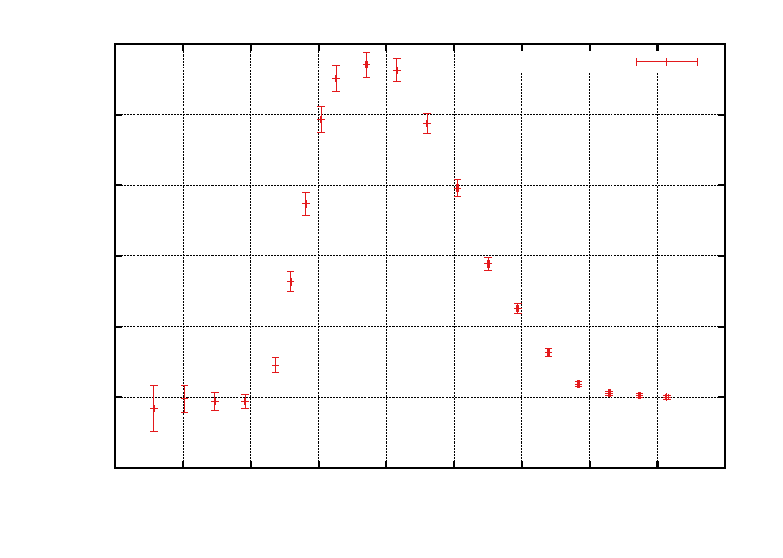
\includegraphics{./plots/thallium_spektrum}}%
    \gplfronttext
  \end{picture}%
\endgroup

	\caption{Spektrum von \isotope[204]{Tl} gemessen bei \SI{4}{\percent} Transmission mit einer Messdauer von \SI{100}{\second}.}
	\label{fig:thallium_spectrum}
\end{figure}

\subsubsection{Bestimmung der Maximalenergie von Thallium}
\label{sssec:kurie_thallium}

Literatur:\\
\url{http://www.nndc.bnl.gov/nudat2/decaysearchdirect.jsp?nuc=204TL&unc=nds}\\
\url{http://www.nndc.bnl.gov/nudat2/decaysearchdirect.jsp?nuc=22NA&unc=nds}\\

Die Bestimmung der Maximalenergie der $\beta$-Spektren erfolgt hier über die Bestimmung des Endpunktes $\epsilon_0$ im Kurie-Diagramm \ref{fig:thallium_kurie}.
In dieser Darstellung wird die Fermi-Funktion von Thallium für verschiedene Impulse $\eta$ beziehungsweise Energien $\epsilon$ benötigt.
Dazu werden die in \cite{anleitung} gegebenen Datenpunkte extrapoliert, indem eine geeignete Kurve an diese angepasst wird.
Als Anpassungshypothese wird gemäß \cite{fermi_function}:
\begin{align}
	F(Z, \epsilon) = \sqrt{A + \frac{B}{\epsilon - 1}}
	\label{eq:hypothese_fermifunktion}
\end{align}
gewählt.
Die Anpassung der Kurve mit \texttt{gnuplot} ergibt:
\begin{align*}
	A &= \num{137.576 +- 3.429} \\
	B &= \num{348.934 +- 0.7867}
\end{align*}
wobei im Folgenden der Fehler der Fermi-Funktion gegenüber der Fehler in den anderen Größen vernachlässigt wird.
Trägt man die angepasste Funktion und die in \cite{anleitung} gegebenen Datenpunkte auf, so erhält man Abbildung \ref{fig:fermi_tl}.
\begin{figure}[h]
	\centering
	% GNUPLOT: LaTeX picture with Postscript
\begingroup
  \makeatletter
  \providecommand\color[2][]{%
    \GenericError{(gnuplot) \space\space\space\@spaces}{%
      Package color not loaded in conjunction with
      terminal option `colourtext'%
    }{See the gnuplot documentation for explanation.%
    }{Either use 'blacktext' in gnuplot or load the package
      color.sty in LaTeX.}%
    \renewcommand\color[2][]{}%
  }%
  \providecommand\includegraphics[2][]{%
    \GenericError{(gnuplot) \space\space\space\@spaces}{%
      Package graphicx or graphics not loaded%
    }{See the gnuplot documentation for explanation.%
    }{The gnuplot epslatex terminal needs graphicx.sty or graphics.sty.}%
    \renewcommand\includegraphics[2][]{}%
  }%
  \providecommand\rotatebox[2]{#2}%
  \@ifundefined{ifGPcolor}{%
    \newif\ifGPcolor
    \GPcolortrue
  }{}%
  \@ifundefined{ifGPblacktext}{%
    \newif\ifGPblacktext
    \GPblacktexttrue
  }{}%
  % define a \g@addto@macro without @ in the name:
  \let\gplgaddtomacro\g@addto@macro
  % define empty templates for all commands taking text:
  \gdef\gplbacktext{}%
  \gdef\gplfronttext{}%
  \makeatother
  \ifGPblacktext
    % no textcolor at all
    \def\colorrgb#1{}%
    \def\colorgray#1{}%
  \else
    % gray or color?
    \ifGPcolor
      \def\colorrgb#1{\color[rgb]{#1}}%
      \def\colorgray#1{\color[gray]{#1}}%
      \expandafter\def\csname LTw\endcsname{\color{white}}%
      \expandafter\def\csname LTb\endcsname{\color{black}}%
      \expandafter\def\csname LTa\endcsname{\color{black}}%
      \expandafter\def\csname LT0\endcsname{\color[rgb]{1,0,0}}%
      \expandafter\def\csname LT1\endcsname{\color[rgb]{0,1,0}}%
      \expandafter\def\csname LT2\endcsname{\color[rgb]{0,0,1}}%
      \expandafter\def\csname LT3\endcsname{\color[rgb]{1,0,1}}%
      \expandafter\def\csname LT4\endcsname{\color[rgb]{0,1,1}}%
      \expandafter\def\csname LT5\endcsname{\color[rgb]{1,1,0}}%
      \expandafter\def\csname LT6\endcsname{\color[rgb]{0,0,0}}%
      \expandafter\def\csname LT7\endcsname{\color[rgb]{1,0.3,0}}%
      \expandafter\def\csname LT8\endcsname{\color[rgb]{0.5,0.5,0.5}}%
    \else
      % gray
      \def\colorrgb#1{\color{black}}%
      \def\colorgray#1{\color[gray]{#1}}%
      \expandafter\def\csname LTw\endcsname{\color{white}}%
      \expandafter\def\csname LTb\endcsname{\color{black}}%
      \expandafter\def\csname LTa\endcsname{\color{black}}%
      \expandafter\def\csname LT0\endcsname{\color{black}}%
      \expandafter\def\csname LT1\endcsname{\color{black}}%
      \expandafter\def\csname LT2\endcsname{\color{black}}%
      \expandafter\def\csname LT3\endcsname{\color{black}}%
      \expandafter\def\csname LT4\endcsname{\color{black}}%
      \expandafter\def\csname LT5\endcsname{\color{black}}%
      \expandafter\def\csname LT6\endcsname{\color{black}}%
      \expandafter\def\csname LT7\endcsname{\color{black}}%
      \expandafter\def\csname LT8\endcsname{\color{black}}%
    \fi
  \fi
    \setlength{\unitlength}{0.0500bp}%
    \ifx\gptboxheight\undefined%
      \newlength{\gptboxheight}%
      \newlength{\gptboxwidth}%
      \newsavebox{\gptboxtext}%
    \fi%
    \setlength{\fboxrule}{0.5pt}%
    \setlength{\fboxsep}{1pt}%
\begin{picture}(7200.00,5040.00)%
    \gplgaddtomacro\gplbacktext{%
      \csname LTb\endcsname%
      \put(814,704){\makebox(0,0)[r]{\strut{}$0$}}%
      \csname LTb\endcsname%
      \put(814,1213){\makebox(0,0)[r]{\strut{}$20$}}%
      \csname LTb\endcsname%
      \put(814,1722){\makebox(0,0)[r]{\strut{}$40$}}%
      \csname LTb\endcsname%
      \put(814,2231){\makebox(0,0)[r]{\strut{}$60$}}%
      \csname LTb\endcsname%
      \put(814,2740){\makebox(0,0)[r]{\strut{}$80$}}%
      \csname LTb\endcsname%
      \put(814,3248){\makebox(0,0)[r]{\strut{}$100$}}%
      \csname LTb\endcsname%
      \put(814,3757){\makebox(0,0)[r]{\strut{}$120$}}%
      \csname LTb\endcsname%
      \put(814,4266){\makebox(0,0)[r]{\strut{}$140$}}%
      \csname LTb\endcsname%
      \put(814,4775){\makebox(0,0)[r]{\strut{}$160$}}%
      \csname LTb\endcsname%
      \put(946,484){\makebox(0,0){\strut{}1{,}0}}%
      \csname LTb\endcsname%
      \put(1727,484){\makebox(0,0){\strut{}1{,}2}}%
      \csname LTb\endcsname%
      \put(2508,484){\makebox(0,0){\strut{}1{,}4}}%
      \csname LTb\endcsname%
      \put(3289,484){\makebox(0,0){\strut{}1{,}6}}%
      \csname LTb\endcsname%
      \put(4070,484){\makebox(0,0){\strut{}1{,}8}}%
      \csname LTb\endcsname%
      \put(4851,484){\makebox(0,0){\strut{}2{,}0}}%
      \csname LTb\endcsname%
      \put(5632,484){\makebox(0,0){\strut{}2{,}2}}%
      \csname LTb\endcsname%
      \put(6413,484){\makebox(0,0){\strut{}2{,}4}}%
    }%
    \gplgaddtomacro\gplfronttext{%
      \csname LTb\endcsname%
      \put(176,2739){\rotatebox{-270}{\makebox(0,0){\strut{}$F(Z = \num{82},\epsilon)$}}}%
      \put(3874,154){\makebox(0,0){\strut{}$\epsilon$}}%
      \csname LTb\endcsname%
      \put(5816,4602){\makebox(0,0)[r]{\strut{}tabellierte Werte}}%
      \csname LTb\endcsname%
      \put(5816,4382){\makebox(0,0)[r]{\strut{}Fermifunktion}}%
    }%
    \gplbacktext
    \put(0,0){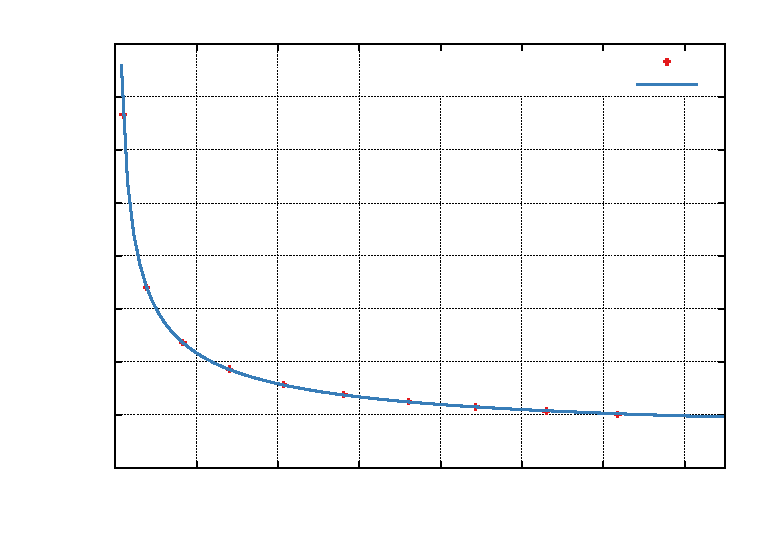
\includegraphics{./plots/fermi_tl}}%
    \gplfronttext
  \end{picture}%
\endgroup

	\caption{Anpassung der Hypothese \eqref{eq:hypothese_fermifunktion} an den in \cite{anleitung} gegebenen Datensatz zur Fermi-Funktion von Thallium.}
	\label{fig:fermi_tl}
\end{figure}
Nun kann die Berechnung des Graphens in der Kurie-Darstellung erfolgen.
Dazu empfiehlt es sich die dimensionslose Darstellung von Impuls $\eta$ und Energie $\epsilon$ zu verwenden.
Zunächst wird dazu aus dem $(B \rho)$-Wert der Tabelle \ref{tab:spektrum_tl} der dimensionslose Impuls gemäß Gleichung \eqref{eq:brho_to_eta} berechnet.
Dementsprechend ergibt sich der Fehler mittels Gauß'scher Fehlerfortpflanzung zu:
\begin{align*}
	\Delta \eta = \frac{\Delta (B \rho)}{\SI{1704.5}{G.cm}}
\end{align*}
Anschließend kann mit der Energie-Impuls-Relation für relativistische Teilchen \eqref{eq:energie_impuls_rel} die dimensionslose Energie $\epsilon$ berechnet werden.
Auch hier ergibt sich der Fehler mit Gauß'scher Fehlefortpflanzung zu:
\begin{align*}
	\Delta \epsilon = \frac{\eta \, \Delta \eta}{\epsilon}
\end{align*}
Schließlich kann die konkrete Kurie-Darstellung berechnet werden:
\begin{align}
	y &= \sqrt{\frac{n}{F(Z,\epsilon) \, \eta \, \epsilon}}
	\label{eq:kurie_y}
\end{align}
und der Fehler berechnet sich zu:
\begin{align}
	\Delta y &= 
	\sqrt{\frac{1}{4 F(Z, \epsilon) \, \eta \, \epsilon}
	\left( \frac{\Delta N^2}{N} + N \frac{\Delta \eta^2}{\eta^2} + N \frac{\Delta \epsilon^2}{\epsilon^2} \right)
	}
\end{align}
Die so berechneten Punkte in dem Kurie-Diagramm wurden in Tabelle \ref{tab:kurie_tl} aufgetragen, dabei ist zu beachten, dass nur die Werte eingetragen sind, für die der Radikand von Gleichung \ref{eq:kurie_y} einen positiven Wert annimmt.
Die Anpassung erfolgt über die Hypothese:
\begin{align}
	y = m (\epsilon - \epsilon_0)
\end{align}
mit den Anpassungsparametern $m$ und $\epsilon_0$.
\begin{figure}[h]
	\centering
	% GNUPLOT: LaTeX picture with Postscript
\begingroup
  \makeatletter
  \providecommand\color[2][]{%
    \GenericError{(gnuplot) \space\space\space\@spaces}{%
      Package color not loaded in conjunction with
      terminal option `colourtext'%
    }{See the gnuplot documentation for explanation.%
    }{Either use 'blacktext' in gnuplot or load the package
      color.sty in LaTeX.}%
    \renewcommand\color[2][]{}%
  }%
  \providecommand\includegraphics[2][]{%
    \GenericError{(gnuplot) \space\space\space\@spaces}{%
      Package graphicx or graphics not loaded%
    }{See the gnuplot documentation for explanation.%
    }{The gnuplot epslatex terminal needs graphicx.sty or graphics.sty.}%
    \renewcommand\includegraphics[2][]{}%
  }%
  \providecommand\rotatebox[2]{#2}%
  \@ifundefined{ifGPcolor}{%
    \newif\ifGPcolor
    \GPcolortrue
  }{}%
  \@ifundefined{ifGPblacktext}{%
    \newif\ifGPblacktext
    \GPblacktexttrue
  }{}%
  % define a \g@addto@macro without @ in the name:
  \let\gplgaddtomacro\g@addto@macro
  % define empty templates for all commands taking text:
  \gdef\gplbacktext{}%
  \gdef\gplfronttext{}%
  \makeatother
  \ifGPblacktext
    % no textcolor at all
    \def\colorrgb#1{}%
    \def\colorgray#1{}%
  \else
    % gray or color?
    \ifGPcolor
      \def\colorrgb#1{\color[rgb]{#1}}%
      \def\colorgray#1{\color[gray]{#1}}%
      \expandafter\def\csname LTw\endcsname{\color{white}}%
      \expandafter\def\csname LTb\endcsname{\color{black}}%
      \expandafter\def\csname LTa\endcsname{\color{black}}%
      \expandafter\def\csname LT0\endcsname{\color[rgb]{1,0,0}}%
      \expandafter\def\csname LT1\endcsname{\color[rgb]{0,1,0}}%
      \expandafter\def\csname LT2\endcsname{\color[rgb]{0,0,1}}%
      \expandafter\def\csname LT3\endcsname{\color[rgb]{1,0,1}}%
      \expandafter\def\csname LT4\endcsname{\color[rgb]{0,1,1}}%
      \expandafter\def\csname LT5\endcsname{\color[rgb]{1,1,0}}%
      \expandafter\def\csname LT6\endcsname{\color[rgb]{0,0,0}}%
      \expandafter\def\csname LT7\endcsname{\color[rgb]{1,0.3,0}}%
      \expandafter\def\csname LT8\endcsname{\color[rgb]{0.5,0.5,0.5}}%
    \else
      % gray
      \def\colorrgb#1{\color{black}}%
      \def\colorgray#1{\color[gray]{#1}}%
      \expandafter\def\csname LTw\endcsname{\color{white}}%
      \expandafter\def\csname LTb\endcsname{\color{black}}%
      \expandafter\def\csname LTa\endcsname{\color{black}}%
      \expandafter\def\csname LT0\endcsname{\color{black}}%
      \expandafter\def\csname LT1\endcsname{\color{black}}%
      \expandafter\def\csname LT2\endcsname{\color{black}}%
      \expandafter\def\csname LT3\endcsname{\color{black}}%
      \expandafter\def\csname LT4\endcsname{\color{black}}%
      \expandafter\def\csname LT5\endcsname{\color{black}}%
      \expandafter\def\csname LT6\endcsname{\color{black}}%
      \expandafter\def\csname LT7\endcsname{\color{black}}%
      \expandafter\def\csname LT8\endcsname{\color{black}}%
    \fi
  \fi
    \setlength{\unitlength}{0.0500bp}%
    \ifx\gptboxheight\undefined%
      \newlength{\gptboxheight}%
      \newlength{\gptboxwidth}%
      \newsavebox{\gptboxtext}%
    \fi%
    \setlength{\fboxrule}{0.5pt}%
    \setlength{\fboxsep}{1pt}%
\begin{picture}(7200.00,5040.00)%
    \gplgaddtomacro\gplbacktext{%
      \csname LTb\endcsname%
      \put(814,975){\makebox(0,0)[r]{\strut{}$0$}}%
      \csname LTb\endcsname%
      \put(814,1518){\makebox(0,0)[r]{\strut{}$0{,}1$}}%
      \csname LTb\endcsname%
      \put(814,2061){\makebox(0,0)[r]{\strut{}$0{,}2$}}%
      \csname LTb\endcsname%
      \put(814,2604){\makebox(0,0)[r]{\strut{}$0{,}3$}}%
      \csname LTb\endcsname%
      \put(814,3147){\makebox(0,0)[r]{\strut{}$0{,}4$}}%
      \csname LTb\endcsname%
      \put(814,3689){\makebox(0,0)[r]{\strut{}$0{,}5$}}%
      \csname LTb\endcsname%
      \put(814,4232){\makebox(0,0)[r]{\strut{}$0{,}6$}}%
      \csname LTb\endcsname%
      \put(814,4775){\makebox(0,0)[r]{\strut{}$0{,}7$}}%
      \csname LTb\endcsname%
      \put(946,484){\makebox(0,0){\strut{}$1$}}%
      \csname LTb\endcsname%
      \put(1678,484){\makebox(0,0){\strut{}$1{,}2$}}%
      \csname LTb\endcsname%
      \put(2410,484){\makebox(0,0){\strut{}$1{,}4$}}%
      \csname LTb\endcsname%
      \put(3142,484){\makebox(0,0){\strut{}$1{,}6$}}%
      \csname LTb\endcsname%
      \put(3874,484){\makebox(0,0){\strut{}$1{,}8$}}%
      \csname LTb\endcsname%
      \put(4607,484){\makebox(0,0){\strut{}$2$}}%
      \csname LTb\endcsname%
      \put(5339,484){\makebox(0,0){\strut{}$2{,}2$}}%
      \csname LTb\endcsname%
      \put(6071,484){\makebox(0,0){\strut{}$2{,}4$}}%
      \csname LTb\endcsname%
      \put(6803,484){\makebox(0,0){\strut{}$2{,}6$}}%
    }%
    \gplgaddtomacro\gplfronttext{%
      \csname LTb\endcsname%
      \put(176,2739){\rotatebox{-270}{\makebox(0,0){\strut{}$y$}}}%
      \put(3874,154){\makebox(0,0){\strut{}$\epsilon$}}%
      \csname LTb\endcsname%
      \put(5816,4602){\makebox(0,0)[r]{\strut{}Messwerte}}%
      \csname LTb\endcsname%
      \put(5816,4382){\makebox(0,0)[r]{\strut{}f(x)}}%
    }%
    \gplbacktext
    \put(0,0){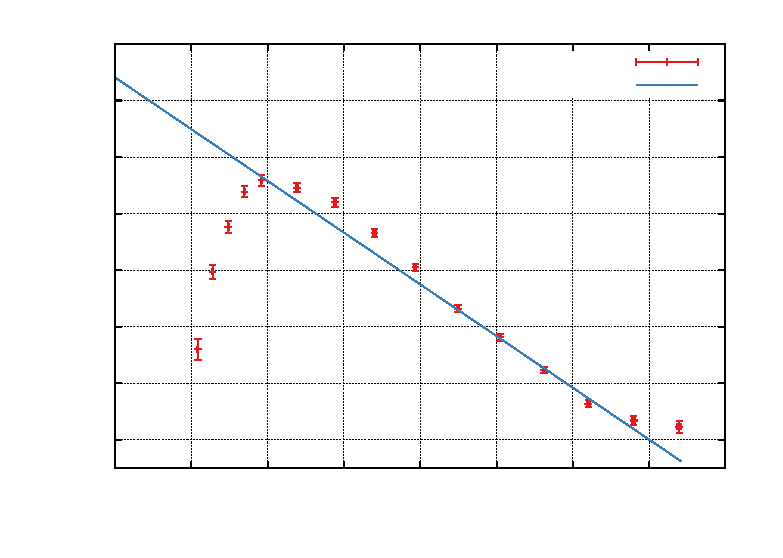
\includegraphics{./plots/thallium_kurie}}%
    \gplfronttext
  \end{picture}%
\endgroup

	\caption{Kurie-Darstellung des Spektrums von \isotope[204]{Tl}. Die Anpassung einer Geraden an den linearen Teil des Graphens (Bereich der Anpassung: $\num{1.8} \leq \epsilon \leq {2.4}$) ergibt den Endpunkt $\epsilon_0 = \num{2.401 +- 0.020}$.}
	\label{fig:thallium_kurie}
\end{figure}
So kann der Endpunkt des Kurie-Diagramms direkt abgelesen werden.
\begin{align}
	m &= \num{-0.457 +- 0.026} \\
	\epsilon_0 &= \num{2.401 +- 0.020}
\end{align}
Aus dem Endpunkt $\epsilon_0$ kann nun die Zerfallsenergie berechnet werden (REF THEORIE):
\begin{align}
	Q = (\epsilon_0 - 1) \cdot m_\mathrm{e} c^2
\end{align}
Mit der Elektronenmasse $m_\mathrm{e} c^2 = \SI{511}{\kilo\electronvolt}$ ergibt sich:
\begin{align}
	Q_\mathrm{Tl} = \SI{716 +- 11}{\kilo\electronvolt}
\end{align}

\subsubsection{Spektrum von Natrium}
\begin{wraptable}{o}{4.7cm}
	\centering
	\begin{tabular}{c}
\toprule
{$N$} \\
\midrule
 37   \\
 52   \\
 45   \\
 51   \\
 45   \\
 36   \\
 54   \\
 44   \\
 48   \\
 49   \\
\midrule
{Mittelwert $N_0$} \\
\num{46.1 +- 6.1} \\
\bottomrule
\end{tabular}

	\caption{Untergrundmessung für \isotope[22]{Na} mit einer Messdauer von \SI{100}{\second} bei \SI{4}{\percent} Transmission.}
	\label{tab:untergrund_na}
\end{wraptable}
Bei der Auswertung des Natrium-Zerfalls wird analog zu den beiden anderen Zerfällen vorgegangen.
Der über \SI{100}{\second} gemessene Untergrund bei \SI{1}{\percent} Transmission ist in Tabelle \ref{tab:untergrund_na} festgehalten worden.
Mit der Korrektur der Hallspannung und nach Abziehen des Untergrunds erhält man das in Abbildung \ref{fig:natrium_spectrum} gezeigte Spektrum für den Zerfall von Natrium.
Die dazu gehörenden Messwerte sind in Tabelle \ref{tab:spektrum_na} notiert.
Hier muss beachtet werden, dass die Hallspannung durchweg ein anderes Vorzeichen hat als bei den anderen Spektren.
Diese wurde in umgekehrter Polung angelegt, da Natrium unter Aussendung eines Positrons zerfällt ($\beta^+$-Zerfall).
\begin{figure}[h]
	\centering
	% GNUPLOT: LaTeX picture with Postscript
\begingroup
  \makeatletter
  \providecommand\color[2][]{%
    \GenericError{(gnuplot) \space\space\space\@spaces}{%
      Package color not loaded in conjunction with
      terminal option `colourtext'%
    }{See the gnuplot documentation for explanation.%
    }{Either use 'blacktext' in gnuplot or load the package
      color.sty in LaTeX.}%
    \renewcommand\color[2][]{}%
  }%
  \providecommand\includegraphics[2][]{%
    \GenericError{(gnuplot) \space\space\space\@spaces}{%
      Package graphicx or graphics not loaded%
    }{See the gnuplot documentation for explanation.%
    }{The gnuplot epslatex terminal needs graphicx.sty or graphics.sty.}%
    \renewcommand\includegraphics[2][]{}%
  }%
  \providecommand\rotatebox[2]{#2}%
  \@ifundefined{ifGPcolor}{%
    \newif\ifGPcolor
    \GPcolortrue
  }{}%
  \@ifundefined{ifGPblacktext}{%
    \newif\ifGPblacktext
    \GPblacktexttrue
  }{}%
  % define a \g@addto@macro without @ in the name:
  \let\gplgaddtomacro\g@addto@macro
  % define empty templates for all commands taking text:
  \gdef\gplbacktext{}%
  \gdef\gplfronttext{}%
  \makeatother
  \ifGPblacktext
    % no textcolor at all
    \def\colorrgb#1{}%
    \def\colorgray#1{}%
  \else
    % gray or color?
    \ifGPcolor
      \def\colorrgb#1{\color[rgb]{#1}}%
      \def\colorgray#1{\color[gray]{#1}}%
      \expandafter\def\csname LTw\endcsname{\color{white}}%
      \expandafter\def\csname LTb\endcsname{\color{black}}%
      \expandafter\def\csname LTa\endcsname{\color{black}}%
      \expandafter\def\csname LT0\endcsname{\color[rgb]{1,0,0}}%
      \expandafter\def\csname LT1\endcsname{\color[rgb]{0,1,0}}%
      \expandafter\def\csname LT2\endcsname{\color[rgb]{0,0,1}}%
      \expandafter\def\csname LT3\endcsname{\color[rgb]{1,0,1}}%
      \expandafter\def\csname LT4\endcsname{\color[rgb]{0,1,1}}%
      \expandafter\def\csname LT5\endcsname{\color[rgb]{1,1,0}}%
      \expandafter\def\csname LT6\endcsname{\color[rgb]{0,0,0}}%
      \expandafter\def\csname LT7\endcsname{\color[rgb]{1,0.3,0}}%
      \expandafter\def\csname LT8\endcsname{\color[rgb]{0.5,0.5,0.5}}%
    \else
      % gray
      \def\colorrgb#1{\color{black}}%
      \def\colorgray#1{\color[gray]{#1}}%
      \expandafter\def\csname LTw\endcsname{\color{white}}%
      \expandafter\def\csname LTb\endcsname{\color{black}}%
      \expandafter\def\csname LTa\endcsname{\color{black}}%
      \expandafter\def\csname LT0\endcsname{\color{black}}%
      \expandafter\def\csname LT1\endcsname{\color{black}}%
      \expandafter\def\csname LT2\endcsname{\color{black}}%
      \expandafter\def\csname LT3\endcsname{\color{black}}%
      \expandafter\def\csname LT4\endcsname{\color{black}}%
      \expandafter\def\csname LT5\endcsname{\color{black}}%
      \expandafter\def\csname LT6\endcsname{\color{black}}%
      \expandafter\def\csname LT7\endcsname{\color{black}}%
      \expandafter\def\csname LT8\endcsname{\color{black}}%
    \fi
  \fi
  \setlength{\unitlength}{0.0500bp}%
  \begin{picture}(7200.00,5040.00)%
    \gplgaddtomacro\gplbacktext{%
      \csname LTb\endcsname%
      \put(946,704){\makebox(0,0)[r]{\strut{}-1}}%
      \csname LTb\endcsname%
      \put(946,1111){\makebox(0,0)[r]{\strut{}-0{,}5}}%
      \csname LTb\endcsname%
      \put(946,1518){\makebox(0,0)[r]{\strut{} 0}}%
      \csname LTb\endcsname%
      \put(946,1925){\makebox(0,0)[r]{\strut{} 0{,}5}}%
      \csname LTb\endcsname%
      \put(946,2332){\makebox(0,0)[r]{\strut{} 1}}%
      \csname LTb\endcsname%
      \put(946,2740){\makebox(0,0)[r]{\strut{} 1{,}5}}%
      \csname LTb\endcsname%
      \put(946,3147){\makebox(0,0)[r]{\strut{} 2}}%
      \csname LTb\endcsname%
      \put(946,3554){\makebox(0,0)[r]{\strut{} 2{,}5}}%
      \csname LTb\endcsname%
      \put(946,3961){\makebox(0,0)[r]{\strut{} 3}}%
      \csname LTb\endcsname%
      \put(946,4368){\makebox(0,0)[r]{\strut{} 3{,}5}}%
      \csname LTb\endcsname%
      \put(946,4775){\makebox(0,0)[r]{\strut{} 4}}%
      \csname LTb\endcsname%
      \put(1078,484){\makebox(0,0){\strut{} 0}}%
      \csname LTb\endcsname%
      \put(1714,484){\makebox(0,0){\strut{} 500}}%
      \csname LTb\endcsname%
      \put(2350,484){\makebox(0,0){\strut{} 1000}}%
      \csname LTb\endcsname%
      \put(2986,484){\makebox(0,0){\strut{} 1500}}%
      \csname LTb\endcsname%
      \put(3622,484){\makebox(0,0){\strut{} 2000}}%
      \csname LTb\endcsname%
      \put(4259,484){\makebox(0,0){\strut{} 2500}}%
      \csname LTb\endcsname%
      \put(4895,484){\makebox(0,0){\strut{} 3000}}%
      \csname LTb\endcsname%
      \put(5531,484){\makebox(0,0){\strut{} 3500}}%
      \csname LTb\endcsname%
      \put(6167,484){\makebox(0,0){\strut{} 4000}}%
      \csname LTb\endcsname%
      \put(6803,484){\makebox(0,0){\strut{} 4500}}%
      \put(176,2739){\rotatebox{-270}{\makebox(0,0){\strut{}$n$}}}%
      \put(3940,154){\makebox(0,0){\strut{}$B \rho$ / \si{G.cm}}}%
    }%
    \gplgaddtomacro\gplfronttext{%
      \csname LTb\endcsname%
      \put(5816,4602){\makebox(0,0)[r]{\strut{}Messwerte}}%
    }%
    \gplbacktext
    \put(0,0){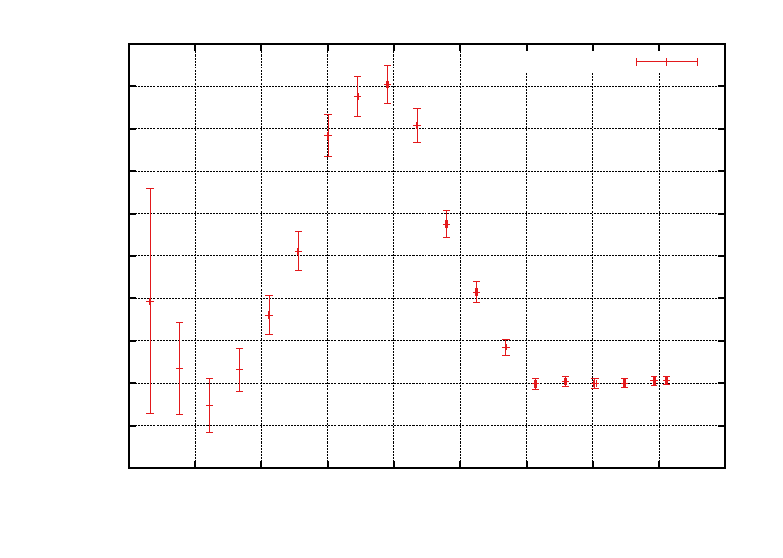
\includegraphics{./plots/natrium_spektrum}}%
    \gplfronttext
  \end{picture}%
\endgroup

	\caption{Spektrum von \isotope[22]{Na} gemessen bei \SI{4}{\percent} Transmission mit einer Messdauer von \SI{100}{\second}.}
	\label{fig:natrium_spectrum}
\end{figure}

\subsubsection{Bestimmung der Endpunktsenergie von Natrium}
Es soll nun die Endpunktsenergie von \isotope[22]{Na} bestimmt werden.
Die Vorgehensweise dazu ist analog zur Bestimmung der Endpunktsenergie von Thallium in Abschnitt \ref{sssec:kurie_thallium} mit Ausnahme, dass die Fermi-Funktion von Natrium direkt aus \cite{riezler} abgelesen wurde.
\begin{align}
	m &= \num{-2.96+- 0.12} \\
	\epsilon_0 &= \num{2.077 +- 0.014}
\end{align}
\begin{align}
	Q_\mathrm{Na} = \SI{550 +- 8}{\kilo\electronvolt}
\end{align}
\begin{figure}[h]
	\centering
	% GNUPLOT: LaTeX picture with Postscript
\begingroup
  \makeatletter
  \providecommand\color[2][]{%
    \GenericError{(gnuplot) \space\space\space\@spaces}{%
      Package color not loaded in conjunction with
      terminal option `colourtext'%
    }{See the gnuplot documentation for explanation.%
    }{Either use 'blacktext' in gnuplot or load the package
      color.sty in LaTeX.}%
    \renewcommand\color[2][]{}%
  }%
  \providecommand\includegraphics[2][]{%
    \GenericError{(gnuplot) \space\space\space\@spaces}{%
      Package graphicx or graphics not loaded%
    }{See the gnuplot documentation for explanation.%
    }{The gnuplot epslatex terminal needs graphicx.sty or graphics.sty.}%
    \renewcommand\includegraphics[2][]{}%
  }%
  \providecommand\rotatebox[2]{#2}%
  \@ifundefined{ifGPcolor}{%
    \newif\ifGPcolor
    \GPcolortrue
  }{}%
  \@ifundefined{ifGPblacktext}{%
    \newif\ifGPblacktext
    \GPblacktexttrue
  }{}%
  % define a \g@addto@macro without @ in the name:
  \let\gplgaddtomacro\g@addto@macro
  % define empty templates for all commands taking text:
  \gdef\gplbacktext{}%
  \gdef\gplfronttext{}%
  \makeatother
  \ifGPblacktext
    % no textcolor at all
    \def\colorrgb#1{}%
    \def\colorgray#1{}%
  \else
    % gray or color?
    \ifGPcolor
      \def\colorrgb#1{\color[rgb]{#1}}%
      \def\colorgray#1{\color[gray]{#1}}%
      \expandafter\def\csname LTw\endcsname{\color{white}}%
      \expandafter\def\csname LTb\endcsname{\color{black}}%
      \expandafter\def\csname LTa\endcsname{\color{black}}%
      \expandafter\def\csname LT0\endcsname{\color[rgb]{1,0,0}}%
      \expandafter\def\csname LT1\endcsname{\color[rgb]{0,1,0}}%
      \expandafter\def\csname LT2\endcsname{\color[rgb]{0,0,1}}%
      \expandafter\def\csname LT3\endcsname{\color[rgb]{1,0,1}}%
      \expandafter\def\csname LT4\endcsname{\color[rgb]{0,1,1}}%
      \expandafter\def\csname LT5\endcsname{\color[rgb]{1,1,0}}%
      \expandafter\def\csname LT6\endcsname{\color[rgb]{0,0,0}}%
      \expandafter\def\csname LT7\endcsname{\color[rgb]{1,0.3,0}}%
      \expandafter\def\csname LT8\endcsname{\color[rgb]{0.5,0.5,0.5}}%
    \else
      % gray
      \def\colorrgb#1{\color{black}}%
      \def\colorgray#1{\color[gray]{#1}}%
      \expandafter\def\csname LTw\endcsname{\color{white}}%
      \expandafter\def\csname LTb\endcsname{\color{black}}%
      \expandafter\def\csname LTa\endcsname{\color{black}}%
      \expandafter\def\csname LT0\endcsname{\color{black}}%
      \expandafter\def\csname LT1\endcsname{\color{black}}%
      \expandafter\def\csname LT2\endcsname{\color{black}}%
      \expandafter\def\csname LT3\endcsname{\color{black}}%
      \expandafter\def\csname LT4\endcsname{\color{black}}%
      \expandafter\def\csname LT5\endcsname{\color{black}}%
      \expandafter\def\csname LT6\endcsname{\color{black}}%
      \expandafter\def\csname LT7\endcsname{\color{black}}%
      \expandafter\def\csname LT8\endcsname{\color{black}}%
    \fi
  \fi
    \setlength{\unitlength}{0.0500bp}%
    \ifx\gptboxheight\undefined%
      \newlength{\gptboxheight}%
      \newlength{\gptboxwidth}%
      \newsavebox{\gptboxtext}%
    \fi%
    \setlength{\fboxrule}{0.5pt}%
    \setlength{\fboxsep}{1pt}%
\begin{picture}(7200.00,5040.00)%
    \gplgaddtomacro\gplbacktext{%
      \csname LTb\endcsname%
      \put(814,975){\makebox(0,0)[r]{\strut{}0{,}0}}%
      \csname LTb\endcsname%
      \put(814,1518){\makebox(0,0)[r]{\strut{}0{,}5}}%
      \csname LTb\endcsname%
      \put(814,2061){\makebox(0,0)[r]{\strut{}1{,}0}}%
      \csname LTb\endcsname%
      \put(814,2604){\makebox(0,0)[r]{\strut{}1{,}5}}%
      \csname LTb\endcsname%
      \put(814,3147){\makebox(0,0)[r]{\strut{}2{,}0}}%
      \csname LTb\endcsname%
      \put(814,3689){\makebox(0,0)[r]{\strut{}2{,}5}}%
      \csname LTb\endcsname%
      \put(814,4232){\makebox(0,0)[r]{\strut{}3{,}0}}%
      \csname LTb\endcsname%
      \put(814,4775){\makebox(0,0)[r]{\strut{}3{,}5}}%
      \csname LTb\endcsname%
      \put(946,484){\makebox(0,0){\strut{}1{,}0}}%
      \csname LTb\endcsname%
      \put(2011,484){\makebox(0,0){\strut{}1{,}2}}%
      \csname LTb\endcsname%
      \put(3076,484){\makebox(0,0){\strut{}1{,}4}}%
      \csname LTb\endcsname%
      \put(4141,484){\makebox(0,0){\strut{}1{,}6}}%
      \csname LTb\endcsname%
      \put(5206,484){\makebox(0,0){\strut{}1{,}8}}%
      \csname LTb\endcsname%
      \put(6271,484){\makebox(0,0){\strut{}2{,}0}}%
    }%
    \gplgaddtomacro\gplfronttext{%
      \csname LTb\endcsname%
      \put(176,2739){\rotatebox{-270}{\makebox(0,0){\strut{}$y$}}}%
      \put(3874,154){\makebox(0,0){\strut{}$\epsilon$}}%
      \csname LTb\endcsname%
      \put(5816,4602){\makebox(0,0)[r]{\strut{}Messwerte}}%
      \csname LTb\endcsname%
      \put(5816,4382){\makebox(0,0)[r]{\strut{}Anpassung}}%
    }%
    \gplbacktext
    \put(0,0){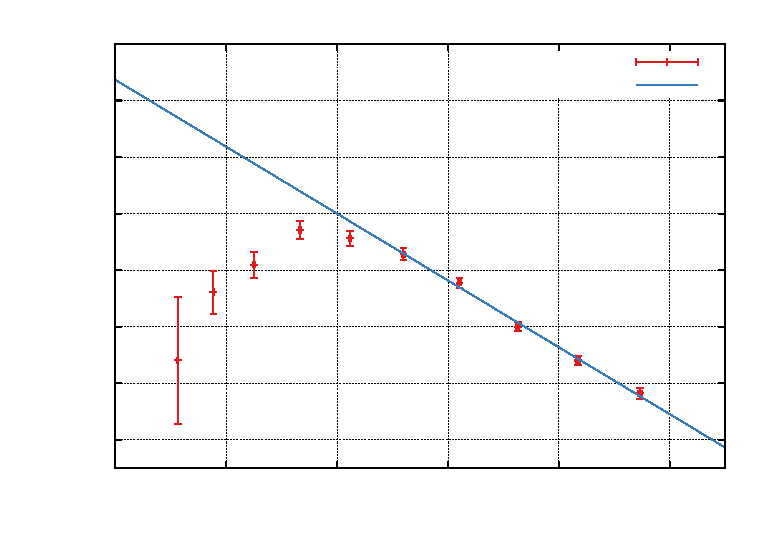
\includegraphics{./plots/natrium_kurie}}%
    \gplfronttext
  \end{picture}%
\endgroup

	\caption{Kurie-Darstellung des Spektrums von \isotope[22]{Na}. Die Anpassung einer Geraden an den linearen Teil des Graphens (Bereich der Anpassung: $\num{1.5} \leq \epsilon \leq {2.0}$) ergibt den Endpunkt $\epsilon_0 = \num{2.077 +- 0.014}$.}
	\label{fig:natrium_kurie}
\end{figure}

\section{Fazit}

\clearpage
% BIBLIOGRAPHIE
\vspace{\fill}
% Maximale Anzahl der Einträge in Klammer
% Zitieren mit \cite{lamport94}
\begin{thebibliography}{19}
\bibitem{krane}
	Kenneth S. Krane,
	\emph{Introductory Nuclear Physics},
	John Wiley \& Sons 1988

\bibitem{mayer-kuckuk}
	Theo Mayer-Kuckuk,
	\emph{Kernphysik - Eine Einführung} (7. Auflage),
	Teubner 2002,

\bibitem{anleitung}
	Physikalisches Praktikum V: Kern- und Teilchenphysik,
	Versuchsbeschreibung \emph{P523: $\beta$-Spektrometer} (Stand: Januar 2015),
	Universität Bonn	

\bibitem{fermi_function}
	Venkataramaiah, P.; Gopala, K.; Basavaraju, A.; Suryanarayana, S.S.; Sanjeevia, H.
	\emph{A simple relation for the Fermi function},
	Journal of Physics G 11 (3): 359-364

\bibitem{riezler}
	Riezler, W.; Kopitzki, K.
	\emph{Kernphysikalisches Praktikum},
	Teubner 1963
 
\end{thebibliography}

\clearpage

% APPENDIX
\begin{appendix}
\section{Anhang}
\begin{sidewaystable}
	\centering
	\begin{tabular}{SSSSSSSSSS}
\toprule
{$U_\mathrm{H}$}  & {$\Delta U_\mathrm{H}$} & {$U_\mathrm{H}^\mathrm{korr.}$} & {$\Delta U_\mathrm{H}^\mathrm{korr.}$} & {$N$}     & {$\Delta N$}   & {$N_\mathrm{korr.}$} & {$\Delta N_\mathrm{korr.}$} & {$n$}     & {$\Delta n$}   \\
\midrule
20.0  & 0.1 & 12.8  & 0.2 & 8.0   & 2.9  & 0.0   & 4.0  & 0.00  & 0.31 \\
30.9  & 0.1 & 23.7  & 0.2 & 8.0   & 2.9  & 0.0   & 4.0  & 0.00  & 0.17 \\
40.1  & 0.1 & 32.9  & 0.2 & 6.0   & 2.5  & -2.0  & 3.8  & -0.06 & 0.12 \\
50.0  & 0.1 & 42.8  & 0.2 & 11.0  & 3.4  & 3.0   & 4.4  & 0.07  & 0.11 \\
60.2  & 0.1 & 53.0  & 0.2 & 34.0  & 5.9  & 26.0  & 6.5  & 0.49  & 0.13 \\
70.1  & 0.1 & 62.9  & 0.2 & 81.0  & 9.0  & 73.0  & 9.5  & 1.16  & 0.15 \\
80.4  & 0.1 & 73.2  & 0.2 & 140.0 & 11.9 & 132.0 & 12.2 & 1.80  & 0.17 \\
89.9  & 0.1 & 82.7  & 0.2 & 143.0 & 12.0 & 135.0 & 12.3 & 1.63  & 0.15 \\
100.1 & 0.1 & 92.9  & 0.2 & 114.0 & 10.7 & 106.0 & 11.1 & 1.14  & 0.12 \\
110.3 & 0.1 & 103.1 & 0.2 & 92.0  & 9.6  & 84.0  & 10.0 & 0.81  & 0.10 \\
120.2 & 0.1 & 113.0 & 0.2 & 60.0  & 7.8  & 52.0  & 8.3  & 0.46  & 0.08 \\
130.0 & 0.1 & 122.8 & 0.2 & 25.0  & 5.0  & 17.0  & 5.8  & 0.14  & 0.05 \\
139.7 & 0.1 & 132.5 & 0.2 & 24.0  & 4.9  & 16.0  & 5.7  & 0.12  & 0.05 \\
150.4 & 0.1 & 143.2 & 0.2 & 23.0  & 4.8  & 15.0  & 5.6  & 0.10  & 0.04 \\
160.1 & 0.1 & 152.9 & 0.2 & 137.0 & 11.8 & 129.0 & 12.1 & 0.84  & 0.08 \\
170.2 & 0.1 & 163.0 & 0.2 & 11.0  & 3.4  & 3.0   & 4.4  & 0.02  & 0.03 \\
180.5 & 0.1 & 173.3 & 0.2 & 7.0   & 2.7  & -1.0  & 3.9  & -0.01 & 0.03 \\
189.8 & 0.1 & 182.6 & 0.2 & 12.0  & 3.5  & 4.0   & 4.5  & 0.02  & 0.03 \\
\bottomrule
\end{tabular}
	\caption{Messdaten des Spektrums von \isotope[137]{Cs} und daraus abgeleitete Größen bei einer Transmission $T = \SI{4}{\percent}$ und Messdauer $t = \SI{40}{s}$.}
	\label{tab:spektrum_ba4_grob}
\end{sidewaystable}

\begin{sidewaystable}
	\centering
	\begin{tabular}{SSSSSSSSSS}
\toprule
{$U_\mathrm{H}$}  & {$\Delta U_\mathrm{H}$} & {$U_\mathrm{H}^\mathrm{korr.}$} & {$\Delta U_\mathrm{H}^\mathrm{korr.}$} & {$N$}     & {$\Delta N$}   & {$N - N_0$} & {$\Delta (N - N_0)$} & {$n$}     & {$\Delta n$}   \\
\midrule
154.9 & 0.1     & 147.7   & 0.2        & 30.0  & 5.5  & 22.0   & 6.2       & 0.15 & 0.05 \\
155.4 & 0.1     & 148.2   & 0.2        & 41.0  & 6.5  & 33.0   & 7.0       & 0.22 & 0.06 \\
156.0 & 0.1     & 148.8   & 0.2        & 41.0  & 6.5  & 33.0   & 7.0       & 0.22 & 0.06 \\
156.5 & 0.1     & 149.3   & 0.2        & 55.0  & 7.5  & 47.0   & 8.0       & 0.31 & 0.07 \\
157.0 & 0.1     & 149.8   & 0.2        & 75.0  & 8.7  & 67.0   & 9.2       & 0.45 & 0.08 \\
157.5 & 0.1     & 150.3   & 0.2        & 115.0 & 10.8 & 107.0  & 11.1      & 0.71 & 0.11 \\
158.0 & 0.1     & 150.8   & 0.2        & 174.0 & 13.2 & 166.0  & 13.5      & 1.10 & 0.15 \\
158.5 & 0.1     & 151.3   & 0.2        & 200.0 & 14.2 & 192.0  & 14.5      & 1.27 & 0.17 \\
159.1 & 0.1     & 151.9   & 0.2        & 181.0 & 13.5 & 173.0  & 13.8      & 1.14 & 0.16 \\
159.5 & 0.1     & 152.3   & 0.2        & 121.0 & 11.0 & 113.0  & 11.4      & 0.74 & 0.11 \\
160.0 & 0.1     & 152.8   & 0.2        & 71.0  & 8.5  & 63.0   & 8.9       & 0.41 & 0.08 \\
160.5 & 0.1     & 153.3   & 0.2        & 64.0  & 8.0  & 56.0   & 8.5       & 0.37 & 0.07 \\
161.0 & 0.1     & 153.8   & 0.2        & 63.0  & 8.0  & 55.0   & 8.5       & 0.36 & 0.07 \\
161.5 & 0.1     & 154.3   & 0.2        & 85.0  & 9.3  & 77.0   & 9.7       & 0.50 & 0.09 \\
162.0 & 0.1     & 154.8   & 0.2        & 94.0  & 9.7  & 86.0   & 10.1      & 0.56 & 0.09 \\
162.5 & 0.1     & 155.3   & 0.2        & 76.0  & 8.8  & 68.0   & 9.2       & 0.44 & 0.08 \\
163.0 & 0.1     & 155.8   & 0.2        & 69.0  & 8.4  & 61.0   & 8.8       & 0.39 & 0.08 \\
163.5 & 0.1     & 156.3   & 0.2        & 60.0  & 7.8  & 52.0   & 8.3       & 0.33 & 0.07 \\
164.0 & 0.1     & 156.8   & 0.2        & 51.0  & 7.2  & 43.0   & 7.7       & 0.27 & 0.06 \\
164.5 & 0.1     & 157.3   & 0.2        & 30.0  & 5.5  & 22.0   & 6.2       & 0.14 & 0.05 \\
165.0 & 0.1     & 157.8   & 0.2        & 23.0  & 4.8  & 15.0   & 5.6       & 0.10 & 0.04 \\
\bottomrule
\end{tabular}
	\caption{Messdaten des Spektrums von \isotope[137]{Cs} im Bereich der \isotope[137]{Ba} Konversionslinien und daraus abgeleitete Größen bei einer Transmission $T = \SI{4}{\percent}$ und Messdauer $t = \SI{40}{s}$.}
	\label{tab:spektrum_ba4_fein}
\end{sidewaystable}

\begin{sidewaystable}
	\centering
	\begin{tabular}{SSSSSSSSSS}
\toprule
{$U_\mathrm{H}$ /}  & {$\Delta U_\mathrm{H}$ /} & {$U_\mathrm{H}^\mathrm{korr.}$ /} & {$\Delta U_\mathrm{H}^\mathrm{korr.}$ /} & {$N$}     & {$\Delta N$}   & {$N_\mathrm{korr.}$} & {$\Delta N_\mathrm{korr.}$} & {$n$}     & {$\Delta n$}   \\
{Skt.} & {Skt.} & {Skt.} & {Skt.} & & & & & & \\  
\midrule
152.9 & 0.1 & 145.7 & 0.2 & 34.0  & 5.9  & 13.9  & 6.4  & 0.10 & 0.05 \\
153.5 & 0.1 & 146.3 & 0.2 & 35.0  & 6.0  & 14.9  & 6.5  & 0.10 & 0.05 \\
154.2 & 0.1 & 147.0 & 0.2 & 38.0  & 6.2  & 17.9  & 6.7  & 0.12 & 0.05 \\
154.5 & 0.1 & 147.3 & 0.2 & 32.0  & 5.7  & 11.9  & 6.3  & 0.08 & 0.05 \\
155.0 & 0.1 & 147.8 & 0.2 & 54.0  & 7.4  & 33.9  & 7.8  & 0.23 & 0.06 \\
155.5 & 0.1 & 148.3 & 0.2 & 55.0  & 7.5  & 34.9  & 7.9  & 0.24 & 0.06 \\
156.0 & 0.1 & 148.8 & 0.2 & 52.0  & 7.3  & 31.9  & 7.7  & 0.21 & 0.06 \\
156.5 & 0.1 & 149.3 & 0.2 & 66.0  & 8.2  & 45.9  & 8.6  & 0.31 & 0.06 \\
157.0 & 0.1 & 149.8 & 0.2 & 104.0 & 10.2 & 83.9  & 10.6 & 0.56 & 0.08 \\
157.4 & 0.1 & 150.2 & 0.2 & 102.0 & 10.1 & 81.9  & 10.5 & 0.55 & 0.07 \\
158.0 & 0.1 & 150.8 & 0.2 & 159.0 & 12.7 & 138.9 & 12.9 & 0.92 & 0.09 \\
158.4 & 0.1 & 151.2 & 0.2 & 175.0 & 13.3 & 154.9 & 13.5 & 1.02 & 0.09 \\
159.0 & 0.1 & 151.8 & 0.2 & 213.0 & 14.6 & 192.9 & 14.9 & 1.27 & 0.10 \\
159.5 & 0.1 & 152.3 & 0.2 & 191.0 & 13.9 & 170.9 & 14.1 & 1.12 & 0.10 \\
160.0 & 0.1 & 152.8 & 0.2 & 88.0  & 9.4  & 67.9  & 9.8  & 0.44 & 0.07 \\
160.5 & 0.1 & 153.3 & 0.2 & 60.0  & 7.8  & 39.9  & 8.2  & 0.26 & 0.06 \\
161.0 & 0.1 & 153.8 & 0.2 & 54.0  & 7.4  & 33.9  & 7.8  & 0.22 & 0.06 \\
161.5 & 0.1 & 154.3 & 0.2 & 71.0  & 8.5  & 50.9  & 8.9  & 0.33 & 0.06 \\
162.0 & 0.1 & 154.8 & 0.2 & 73.0  & 8.6  & 52.9  & 9.0  & 0.34 & 0.06 \\
162.5 & 0.1 & 155.3 & 0.2 & 94.0  & 9.7  & 73.9  & 10.1 & 0.48 & 0.07 \\
163.0 & 0.1 & 155.8 & 0.2 & 97.0  & 9.9  & 76.9  & 10.2 & 0.49 & 0.07 \\
163.5 & 0.1 & 156.3 & 0.2 & 87.0  & 9.4  & 66.9  & 9.7  & 0.43 & 0.07 \\
164.0 & 0.1 & 156.8 & 0.2 & 77.0  & 8.8  & 56.9  & 9.2  & 0.36 & 0.06 \\
164.5 & 0.1 & 157.3 & 0.2 & 53.0  & 7.3  & 32.9  & 7.8  & 0.21 & 0.05 \\
165.0 & 0.1 & 157.8 & 0.2 & 58.0  & 7.7  & 37.9  & 8.1  & 0.24 & 0.06 \\
165.5 & 0.1 & 158.3 & 0.2 & 38.0  & 6.2  & 17.9  & 6.7  & 0.11 & 0.05 \\
166.1 & 0.1 & 158.9 & 0.2 & 30.0  & 5.5  & 9.9   & 6.1  & 0.06 & 0.04 \\
166.6 & 0.1 & 159.4 & 0.2 & 41.0  & 6.5  & 20.9  & 7.0  & 0.13 & 0.05 \\
167.1 & 0.1 & 159.9 & 0.2 & 36.0  & 6.0  & 15.9  & 6.6  & 0.10 & 0.05 \\
167.5 & 0.1 & 160.3 & 0.2 & 46.0  & 6.8  & 25.9  & 7.3  & 0.16 & 0.05 \\
168.1 & 0.1 & 160.9 & 0.2 & 36.0  & 6.0  & 15.9  & 6.6  & 0.10 & 0.05 \\
\bottomrule
\end{tabular}
	\caption{Messdaten des Spektrums von \isotope[137]{Cs} im Bereich der \isotope[137]{Ba} Konversionslinien und daraus abgeleitete Größen bei einer Transmission $T = \SI{4}{\percent}$ und Messdauer $t = \SI{100}{s}$.}
	\label{tab:spektrum_ba1_fein}
\end{sidewaystable}

\begin{sidewaystable}
	\centering
	\begin{tabular}{SSSSSSSSSSSS}
\toprule
{$U_\mathrm{H}$ /}  & {$\Delta U_\mathrm{H}$ /} & {$U_\mathrm{H}^\mathrm{korr.}$ /} & {$\Delta U_\mathrm{H}^\mathrm{korr.}$ /} & {$B \rho$ /} & {$\Delta (B \rho)$ /} & {$N$}     & {$\Delta N$}   & {$N_\mathrm{korr.}$} & {$\Delta N_\mathrm{korr.}$} & {$n$}     & {$\Delta n$}   \\
{Skt.} & {Skt.} & {Skt.} & {Skt.} & {\si{G.cm}} & {\si{G.cm}} & & & & & & \\  
\midrule
19.9  & 0.1 & 12.7  & 0.2 & 285.1  & 2.5 & 43.0  & 6.6  & -4.0  & 8.4  & -0.31 & 0.66 \\ 
30.0  & 0.1 & 22.8  & 0.2 & 511.0  & 2.7 & 46.0  & 6.8  & -1.0  & 8.6  & -0.04 & 0.38 \\
40.0  & 0.1 & 32.8  & 0.2 & 734.8  & 3.0 & 43.0  & 6.6  & -4.0  & 8.4  & -0.12 & 0.26 \\
50.0  & 0.1 & 42.8  & 0.2 & 958.5  & 3.3 & 42.0  & 6.5  & -5.0  & 8.4  & -0.12 & 0.20 \\
60.0  & 0.1 & 52.8  & 0.2 & 1182.2 & 3.6 & 95.0  & 9.8  & 48.0  & 11.1 & 0.91  & 0.21 \\
65.0  & 0.1 & 57.8  & 0.2 & 1294.1 & 3.8 & 236.0 & 15.4 & 189.0 & 16.3 & 3.27  & 0.29 \\
70.0  & 0.1 & 62.8  & 0.2 & 1406.0 & 4.0 & 391.0 & 19.8 & 344.0 & 20.5 & 5.47  & 0.33 \\
75.0  & 0.1 & 67.8  & 0.2 & 1517.8 & 4.2 & 580.0 & 24.1 & 533.0 & 24.7 & 7.86  & 0.37 \\
80.0  & 0.1 & 72.8  & 0.2 & 1629.7 & 4.4 & 704.0 & 26.6 & 657.0 & 27.1 & 9.02  & 0.38 \\
90.0  & 0.1 & 82.8  & 0.2 & 1853.4 & 4.8 & 827.0 & 28.8 & 780.0 & 29.3 & 9.42  & 0.36 \\
100.0 & 0.1 & 92.8  & 0.2 & 2077.2 & 5.3 & 906.0 & 30.1 & 859.0 & 30.6 & 9.25  & 0.33 \\
110.0 & 0.1 & 102.8 & 0.2 & 2300.9 & 5.7 & 844.0 & 29.1 & 797.0 & 29.6 & 7.75  & 0.29 \\
120.0 & 0.1 & 112.8 & 0.2 & 2524.6 & 6.2 & 715.0 & 26.8 & 668.0 & 27.3 & 5.92  & 0.25 \\
130.1 & 0.1 & 122.9 & 0.2 & 2750.6 & 6.7 & 511.0 & 22.7 & 464.0 & 23.3 & 3.77  & 0.19 \\
139.9 & 0.1 & 132.7 & 0.2 & 2969.9 & 7.1 & 381.0 & 19.6 & 334.0 & 20.3 & 2.52  & 0.16 \\
150.0 & 0.1 & 142.8 & 0.2 & 3195.8 & 7.6 & 228.0 & 15.1 & 181.0 & 16.0 & 1.27  & 0.12 \\
159.9 & 0.1 & 152.7 & 0.2 & 3417.3 & 8.1 & 104.0 & 10.2 & 57.0  & 11.5 & 0.37  & 0.08 \\
170.0 & 0.1 & 162.8 & 0.2 & 3643.3 & 8.5 & 66.0  & 8.2  & 19.0  & 9.7  & 0.12  & 0.06 \\
180.0 & 0.1 & 172.8 & 0.2 & 3867.0 & 9.0 & 57.0  & 7.6  & 10.0  & 9.2  & 0.06  & 0.06 \\
189.0 & 0.1 & 181.8 & 0.2 & 4068.4 & 9.5 & 47.0  & 6.9  & 0.0   & 8.7  & 0.00  & 0.05 \\
\bottomrule
\end{tabular}
	\caption{Messdaten des Spektrums von \isotope[204]{Tl} und daraus abgeleitete Größen bei einer Transmission $T = \SI{4}{\percent}$ und Messdauer $t = \SI{100}{s}$.}
	\label{tab:spektrum_tl}
\end{sidewaystable}

\begin{sidewaystable}
	\centering
	\begin{tabular}{SSSSSSSSSSS}
\toprule
{$(B \rho)$ /} & {$\Delta(B \rho)$ /} & {$\eta$}    & {$\Delta \eta$} & {$\epsilon$} & {$\Delta \epsilon$} & {$n$}    & {$\Delta n$}   & {$F(Z, \eta)$}    & {$y$}     & {$\Delta y$}    \\
	{\si{G.cm}} & {\si{G.cm}} & & & & & & & & & \\
\midrule
1182.2 & 3.6      & 0.6936 & 0.0021 & 1.2170  & 0.0012    & 0.91 & 0.21 & 41.8 & 0.160 & 0.019 \\
1294.1 & 3.8      & 0.7592 & 0.0023 & 1.2556  & 0.0014    & 3.27 & 0.29 & 38.8 & 0.297 & 0.013 \\
1406.0 & 4.0      & 0.8249 & 0.0024 & 1.2963  & 0.0015    & 5.47 & 0.33 & 36.3 & 0.376 & 0.012 \\
1517.8 & 4.2      & 0.8905 & 0.0025 & 1.3390  & 0.0017    & 7.86 & 0.37 & 34.2 & 0.439 & 0.011 \\
1629.7 & 4.4      & 0.9561 & 0.0026 & 1.3835  & 0.0018    & 9.02 & 0.38 & 32.4 & 0.459 & 0.010 \\
1853.4 & 4.8      & 1.0874 & 0.0029 & 1.4773  & 0.0021    & 9.42 & 0.36 & 29.5 & 0.446 & 0.009 \\
2077.2 & 5.3      & 1.2186 & 0.0031 & 1.5764  & 0.0024    & 9.25 & 0.33 & 27.3 & 0.420 & 0.008 \\
2300.9 & 5.7      & 1.3499 & 0.0034 & 1.6800  & 0.0027    & 7.75 & 0.29 & 25.5 & 0.366 & 0.007 \\
2524.6 & 6.2      & 1.4812 & 0.0036 & 1.7871  & 0.0030    & 5.92 & 0.25 & 24.1 & 0.305 & 0.007 \\
2750.6 & 6.7      & 1.6137 & 0.0039 & 1.8985  & 0.0033    & 3.77 & 0.19 & 22.9 & 0.232 & 0.006 \\
2969.9 & 7.1      & 1.7424 & 0.0042 & 2.0089  & 0.0036    & 2.52 & 0.16 & 22.0 & 0.181 & 0.006 \\
3195.8 & 7.6      & 1.8749 & 0.0045 & 2.1250  & 0.0040    & 1.27 & 0.12 & 21.2 & 0.123 & 0.006 \\
3417.3 & 8.1      & 2.0049 & 0.0047 & 2.2404  & 0.0043    & 0.37 & 0.08 & 20.5 & 0.064 & 0.007 \\
3643.3 & 8.5      & 2.1375 & 0.0050 & 2.3598  & 0.0046    & 0.12 & 0.06 & 19.9 & 0.034 & 0.009 \\
3867.0 & 9.0      & 2.2687 & 0.0053 & 2.4793  & 0.0049    & 0.06 & 0.06 & 19.3 & 0.023 & 0.011 \\
\bottomrule
\end{tabular}
	\caption{Kurie Tl}
	\label{tab:kurie_tl}
\end{sidewaystable}

\begin{sidewaystable}
	\centering
	\begin{tabular}{SSSSSSSSSSSS}
\toprule
{$U_\mathrm{H}$}  & {$\Delta U_\mathrm{H}$} & {$U_\mathrm{H}^\mathrm{korr.}$} & {$\Delta U_\mathrm{H}^\mathrm{korr.}$} & {$B \rho$} & {$\Delta (B \rho)$} & {$N$}     & {$\Delta N$}   & {$N_\mathrm{korr.}$} & {$\Delta N_\mathrm{korr.}$} & {$n$}     & {$\Delta n$}   \\
\midrule
0.0    & 0.1     & -7.2    & 0.2        & 160.2  & 2.5      & 53.0  & 7.3  & 6.9    & 9.5       & 0.96  & 1.33 \\
-9.9   & 0.1     & -17.1   & 0.2        & 381.7  & 2.6      & 49.0  & 7.0  & 2.9    & 9.3       & 0.17  & 0.55 \\
-20.0  & 0.1     & -27.2   & 0.2        & 607.6  & 2.8      & 39.0  & 6.3  & -7.1   & 8.8       & -0.26 & 0.33 \\
-30.1  & 0.1     & -37.3   & 0.2        & 833.6  & 3.1      & 52.0  & 7.3  & 5.9    & 9.5       & 0.16  & 0.26 \\
-40.1  & 0.1     & -47.3   & 0.2        & 1057.3 & 3.4      & 84.0  & 9.2  & 37.9   & 11.1      & 0.80  & 0.24 \\
-50.0  & 0.1     & -57.2   & 0.2        & 1278.8 & 3.8      & 135.0 & 11.7 & 88.9   & 13.2      & 1.56  & 0.23 \\
-60.0  & 0.1     & -67.2   & 0.2        & 1502.6 & 4.2      & 242.0 & 15.6 & 195.9  & 16.8      & 2.92  & 0.25 \\
-70.0  & 0.1     & -77.2   & 0.2        & 1726.3 & 4.6      & 307.0 & 17.6 & 260.9  & 18.6      & 3.38  & 0.25 \\
-80.0  & 0.1     & -87.2   & 0.2        & 1950.0 & 5.0      & 353.0 & 18.8 & 306.9  & 19.8      & 3.52  & 0.23 \\
-90.0  & 0.1     & -97.2   & 0.2        & 2173.8 & 5.5      & 341.0 & 18.5 & 294.9  & 19.5      & 3.04  & 0.21 \\
-100.0 & 0.1     & -107.2  & 0.2        & 2397.5 & 5.9      & 247.0 & 15.8 & 200.9  & 16.9      & 1.87  & 0.16 \\
-110.0 & 0.1     & -117.2  & 0.2        & 2621.2 & 6.4      & 172.0 & 13.2 & 125.9  & 14.5      & 1.07  & 0.13 \\
-120.0 & 0.1     & -127.2  & 0.2        & 2845.0 & 6.8      & 100.0 & 10.0 & 53.9   & 11.8      & 0.42  & 0.10 \\
-130.0 & 0.1     & -137.2  & 0.2        & 3068.7 & 7.3      & 45.0  & 6.8  & -1.1   & 9.1       & -0.01 & 0.07 \\
-140.0 & 0.1     & -147.2  & 0.2        & 3292.4 & 7.8      & 49.0  & 7.0  & 2.9    & 9.3       & 0.02  & 0.07 \\
-150.0 & 0.1     & -157.2  & 0.2        & 3516.2 & 8.3      & 45.0  & 6.8  & -1.1   & 9.1       & -0.01 & 0.06 \\
-160.0 & 0.1     & -167.2  & 0.2        & 3739.9 & 8.7      & 46.0  & 6.8  & -0.1   & 9.2       & 0.00  & 0.06 \\
-170.0 & 0.1     & -177.2  & 0.2        & 3963.6 & 9.2      & 51.0  & 7.2  & 4.9    & 9.4       & 0.03  & 0.06 \\
-174.1 & 0.1     & -181.3  & 0.2        & 4055.4 & 9.4      & 52.0  & 7.3  & 5.9    & 9.5       & 0.03  & 0.06 \\ 
\bottomrule
\end{tabular}
	\caption{Messdaten des Spektrums von \isotope[22]{Na} und daraus abgeleitete Größen bei einer Transmission $T = \SI{4}{\percent}$ und Messdauer $t = \SI{100}{s}$.}
	\label{tab:spektrum_na}
\end{sidewaystable}

\end{appendix}

\end{document}
